To assess the merits of the feature-family-based strategy, initially the key
aspects of its implementation (Section~\ref{subsec:reana}) are highlighted,
followed by its complexity analysis (Section~\ref{subsec:analyticalComplexity}).
Finally an empirical evaluation (Section~\ref{subsec:empiricalEvaluation}), the
threats to its validity (Section~\ref{sec:threatsValidity}) are presented.


%%%%%%%%%%%%%%%%%%%%%%%%%%%%%%%%%%%%%%%%%%%%%%%%%%%%%%%%%%%%%%%%%%%%%%%%%%%%%%%%
%% IMPLEMENTATION
%%%%%%%%%%%%%%%%%%%%%%%%%%%%%%%%%%%%%%%%%%%%%%%%%%%%%%%%%%%%%%%%%%%%%%%%%%%%%%%%
\section{Implementation   \label{subsec:reana}}


The evaluation method presented hereby is implemented as a new tool named
\textsc{ReAna} (\textbf{Re}liability \textbf{Ana}lysis), whose source code is
open and publicly available\footnote{https://github.com/SPLMC/reana-spl}.
\textsc{ReAna} takes as input a UML behavioral model, for example, built using
the MagicDraw tool\footnote{http://www.nomagic.com/products/magicdraw.html}, and
a feature model described in conjunctive normal form (CNF), for example, as
exported by FeatureIDE~\cite{featureide}. It then outputs the ADD representing
the reliability of all products of the product line to a file in DOT format, and
it prints a list of configurations and respective reliabilities. The latter can
be suppressed or filtered to a subset of possible configurations of interest.

\textsc{ReAna} uses PARAM 2.3~\cite{Hahn_param_2010} to perform parametric model
checking and the CUDD 2.5.1
library\footnote{ftp://vlsi.colorado.edu/pub/cudd-2.5.1.tar.gz} for ADD
manipulation. However, any other tool or library providing the same
functionality (e.g., the parametric model checker from
\citet{Filieri_pmctool_2012}) could be used, too.

\textsc{ReAna}'s main evaluation routine is depicted in
Listing~\ref{lst:evaluate-reliability}. After parsing and transforming the input
models into an RDG structure (see Section~\ref{subsec:transformation}), the
method \texttt{evalReliability} is invoked on the RDG's root node.  Its first
task is to perform a topological sort of the RDG nodes, so that it obtains a
list in which every node comes after all the nodes on which it (transitively)
depends (Line~\ref{line:topological-sort}).  This implements the recursion
described in Section~\ref{sec:familyBasedAnalysis} in an iterative fashion.

\begin{lstlisting}[label={lst:evaluate-reliability},
                   caption={\textsc{ReAna}'s main evaluation routine},
                   float,
                   breaklines,
		   belowcaptionskip=0.1cm]
ADD evalReliability(RDGNode root) {
    List<RDGNode> deps = root.topoSortTransitiveDeps(); (*@\label{line:topological-sort}@*)
    LinkedHashMap<RDGNode, String> expressionsByNode = getReliabilityExpressions(deps); (*@\label{line:model-checking}@*)
    Map<RDGNode, ADD> reliabilities = evalReliabilities(expressionsByNode); (*@\label{line:evaluation}@*)
    return reliabilities.get(root);
}
\end{lstlisting}

Then, it proceeds to parametric model checking of the reliability property in
the FDTMC corresponding to each of the nodes (Line~\ref{line:model-checking}).
Although this step does not depend on the ordering of nodes (because it handles
dependencies as variables), it is useful that its output respects this order.
This way, the resulting reliability expressions ($\varepsilon$ in
Section~\ref{sec:featureBasedAnalysis}) can be evaluated in an order that
allows every variable to be immediately resolved to a previously computed value,
thus eliminating the need for recursion and null checking.


\begin{lstlisting}[label={lst:node-reliability}, 
                   caption={Evaluation of the reliability function for a single node},
                   float,
		   belowcaptionskip=0.1cm] 
ADD evalNodeReliability(RDGNode node,
                          String reliabilityExpression,
                          Map<RDGNode, ADD> relCache) {
    Map<String, ADD> depsReliabilities = new HashMap();
    for (RDGNode dep: node.getDependencies()) {
        ADD depReliability = relCache.get(dep);(*@\label{line:reliability-cache}@*)
        ADD presCond = dep.getPresenceCondition();
        ADD phi = presCond.ifThenElse(depReliability,(*@\label{line:phi}@*)
                                         constantAdd(1));
        depsReliabilities.put(dep.getId(), phi);
    }
    ADD reliability = solve(reliabilityExpression,(*@\label{line:expression-solving}@*)
                               depsReliabilities);
    return FM.times(reliability);(*@\label{line:pruning}@*)
}
\end{lstlisting}


The third step is to evaluate each reliability expression, which yields an ADD
representing the reliability function ($\alpha$ in
Section~\ref{sec:familyBasedAnalysis}) for each of the nodes. The evaluation
of such reliability ADDs (method \texttt{evalReliabilities} in
Line~\ref{line:evaluation}, Listing~\ref{lst:evaluate-reliability}) invokes, for
each node, method \texttt{evalNodeReliability}, which we present in
Listing~\ref{lst:node-reliability}. It computes the $\varphi$ functions of a
node's dependencies (as in Section~\ref{sec:familyBasedAnalysis}), encoding
satisfaction of their presence conditions by means of conditionals in ADD
\texttt{ITE} (\emph{if-then-else}) operations (Line~\ref{line:phi},
Listing~\ref{lst:node-reliability}). The reliability function of each dependency
is looked up in a reliability cache (\texttt{relCache}, in
Line~\ref{line:reliability-cache}, Listing~\ref{lst:node-reliability}) and is
then used as the \emph{consequent} argument of the \texttt{ITE} operator, with
the \emph{alternative} argument being the constant ADD corresponding to $1$.
 
After all these functions are computed, they are used to evaluate the lifted
reliability expression (Line~\ref{line:expression-solving},
Listing~\ref{lst:node-reliability}). Whenever a variable appears in this
expression, function $\varphi$ of the corresponding RDG node (on which the
current one depends) is looked up in a variable--value mapping, indexed by the
node id (\texttt{depsReliabilities}).

When this evaluation of $\alpha$ is done, it is necessary to consider only the
valid configurations for the node at hand by discarding the reliability values
of ill-formed products.  The feature model's rules are represented by an ADD
where all paths leading to terminal 1 represent a valid configuration, otherwise
the path leads to terminal 0. Thus, for the node under evaluation the invalid
configurations are pruned by multiplying its reliability ADD by the one
representing the feature-model's rules (Line~\ref{line:pruning},
Listing~\ref{lst:node-reliability}), so the resulting ADD yields the value 0,
for ill-formed products and the actual reliability for the valid ones.

%When this evaluation of $f$ is done, we prune invalid configurations for the
%node at hand, by multiplying its reliability ADD by the one representing the
%feature model's rules (Line~\ref{line:pruning},
%Listing~\ref{lst:node-reliability}). This way, the resulting ADD yields the
%value 0, for invalid configurations, and the actual reliability, for valid
%ones.

All reliabilities computed in this way are progressively added to the
reliability cache \emph{relCache}. At the end of this loop inside
\texttt{evalReliabilities}, the cache contains the reliability function for
every node and is then returned (Line \ref{line:evaluation},
Listing~\ref{lst:evaluate-reliability}). The reliability of interest is then the
one of the root RDG node (the one argument to \texttt{evalReliability},
Listing~\ref{lst:evaluate-reliability}), so it is queried in constant time
because of the underlying data structure.





%%%%%%%%%%%%%%%%%%%%%%%%%%%%%%%%%%%%%%%%%%%%%%%%%%%%%%%%%%%%%%%%%%%%%%%%%%%%%%%%
%% ANALYTICAL COMPLEXITY
%%%%%%%%%%%%%%%%%%%%%%%%%%%%%%%%%%%%%%%%%%%%%%%%%%%%%%%%%%%%%%%%%%%%%%%%%%%%%%%%
\section{Analytical Complexity \label{subsec:analyticalComplexity}}

The overall analysis time is the sum of the time taken by each of the sequential
steps in Listing~\ref{lst:evaluate-reliability}.  First, the computation of an
ordering that respects the transitive closure of the dependency relation in an
RDG (Line~\ref{line:topological-sort}) is an instance of the classical
topological sorting problem for directed acyclic graphs, which is linear in the
sum of nodes and edges~\citep{CormenAlgorithms}.

Second, the computation of the reliability expression for an RDG node consists
of a call to the PARAM parametric model checker, which requires $n$ calls to
cover all nodes (Line~\ref{line:model-checking}).  The parametric model checking
problem for a model of $s$ states consists of $O(s^3)$ operations over
polynomials, each of which depends on the number of monomials in each operand
\cite{HahnHZ10}.  This number of monomials is, in the worst case, exponential in
the number of existing variables.  The number of variables for a given node is,
in turn, dependent on its number of child nodes and on the modeled behavior
(e.g., if there are loops or alternative paths).  Thus, the time complexity of
computing all the reliability expressions is linear in the number of RDG nodes,
but depends on the topologies of the RDG and of the models represented by each
of its nodes (such dependencies are addressed with more details later on).

Last, method  \texttt{evalReliabilities} calls method
\texttt{evalNodeReliability}, which corresponds to the reliability function
$\alpha$ in Section~\ref{sec:familyBasedAnalysis}, once for each node.
\texttt{evalNodeReliability}'s complexity is dominated by that of ADD
operations, which are polynomial in the size of the operands~\cite{Iris1993}.
Indeed, for ADDs $f$, $g$, and $h$, the \emph{if-then-else} operation
$\texttt{ITE}(f, g, h)$ is $O(|f| \cdot |g| \cdot |h|)$.  Likewise,
$\texttt{APPLY}(f, g, \odot)$, where $\odot$ is a binary ADD operator (e.g.,
multiplication), is $O(|f| \cdot |g|)$.  Here, $|f|$ denotes the size of the ADD
$f$, that is, its number of nodes.  Because of configuration pruning
(Section~\ref{sec:familyBasedAnalysis}), all ADD sizes in our approach are
bound by $|\mathit{FM_{ADD}}|$ (i.e., the size of the ADD that encodes the rules
in the feature model).

Since the evaluation of $\alpha$ for a given node comprises a number of
operations on the reliability ADDs of the nodes on which it depends
(Listing~\ref{lst:node-reliability}, Line~\ref{line:expression-solving}), an
upper bound estimate for polynomial arithmetics must be provide.  If a node
identified by $x$ has $c$ children (nodes on which it depends), $\varepsilon(x)$
is a polynomial in $c$ variables and it has, at most, $e_{\mathit{max}}^c$
monomials of $c$ variables each, where $e_{\mathit{max}}$ is the maximum
exponent for any variable.  Each monomial has in turn, at most, $2c$ operations:
$c$ exponentiations and $c$ multiplications among variables and the coefficient.
Also, no variable can have an exponent greater than the maximum number of
transitions between the initial and the success states of the original FDTMC,
and this number is itself bound by the number $m$ of messages in the
corresponding behavioral model fragment.  Thus, the number of ADD operations
needed to compute this reliability ADD is $O(c \cdot m^c)$.  This leads to an
evaluation time of $O(c \cdot m^c \cdot |\mathit{FM_{ADD}}|^2)$.

Since the reliability of each RDG node needs to be evaluated exactly once (due
to caching), there are $n$ computations of $\alpha(x_i)$, one for each of the
$n$ RDG nodes $x_i$. Hence, the cumulative time spent on reliability functions
computation is ${O(n \cdot c_{\mathit{max}} \cdot
m_{\mathit{max}}^{c_{\mathit{max}}} \cdot |\mathit{FM_{ADD}}|^2)}$, where
$c_{\mathit{max}}$ is the maximum number of children per node, and
$m_{\mathit{max}}$ is the maximum number of messages per model fragment.

Although this complexity bound is quadratic in the number of features, the
number of nodes in an ADD is, in the worst case, exponential in the number of
variables.  As the variables in $\mathit{FM_{ADD}}$ represent features, this
means $|\mathit{FM_{ADD}}|$ can be exponential in the number $F$ of features.
Hence, the worst-case complexity is $O(n \cdot c_{\mathit{max}} \cdot
m_{\mathit{max}}^{c_{\mathit{max}}} \cdot 2^{2 \cdot F})$.  This worst-case
exponential blowup cannot be avoided theoretically, but, in practice, efficient
heuristics can be applied for defining an ordering of variables that can cause
the ADD's size to grow linearly or polynomially, depending on the functions
being represented \cite{baier_principles_2008}.  Thus, as the growth in the
sizes of ADDs varies with the product line being
analyzed~\cite{liang_sat-based_2015} and is, at least, linear in the number of
features, it can also state the best-case time complexity is $O(n \cdot
c_{\mathit{max}} \cdot m_{\mathit{max}}^{c_{\mathit{max}}} \cdot F^2)$.

\begin{framed} In summary, the time complexity of the feature-family-based
	analysis strategy lies between $O(n \cdot c_{\mathit{max}} \cdot
	m_{\mathit{max}}^{c_{\mathit{max}}} \cdot F^2)$ and $O(n \cdot
	c_{\mathit{max}} \cdot m_{\mathit{max}}^{c_{\mathit{max}}} \cdot 2^{2
	\cdot F})$, where $n$ is the number of RDG nodes, $c_{max}$ is the
	maximum number of child nodes in an RDG node, $m_{max}$ is the maximum
	number of messages in a behavioral fragment, and $F$ is the number of
	features of the product line.  
\end{framed}








%%%%%%%%%%%%%%%%%%%%%%%%%%%%%%%%%%%%%%%%%%%%%%%%%%%%%%%%%%%%%%%%%%%%%%%%%%%%%%%%
%% EMPIRICAL EVALUATION
%%%%%%%%%%%%%%%%%%%%%%%%%%%%%%%%%%%%%%%%%%%%%%%%%%%%%%%%%%%%%%%%%%%%%%%%%%%%%%%%

\section{Empirical Evaluation \label{subsec:empiricalEvaluation}}


The empirical evaluation aims at comparing the feature-family-based analysis
strategy (c.f. Chapter \ref{chp:featureFamilyBasedAnalysis}) with other
state-of-the-art strategies for product-line reliability analysis, as identified
by \citet{thum_classification_2014}: product-based, family-based,
fea\-ture-prod\-uct-based, and fam\-i\-ly-prod\-uct-based. It is expected that
the feature-family-based approach performs better than the others, since it (a)
decomposes behavioral models into smaller ones and (b) prevents an exponential
blowup by computing the reliabilities of all products at once using ADDs. The
comparison focuses on the practical complexity of the selected strategies and is
guided by the following research question:

\begin{itemize} 
  \item \textbf{RQ1:} How do product-line reliability analysis strategies
	  compare to one another in terms of time and space?
  %% \item \textbf{RQ1:} What is the \textit{practical time complexity} for
  %%   evaluating the reliability of a whole product line?  
  %% \item \textbf{RQ2:} What is the \textit{practical space complexity} for
  %%   evaluating the reliability of a whole product line?  
\end{itemize}


To address RQ1, it was measured the time and space demanded by each strategy for
the analysis of six available software product lines and augmented versions
thereof.  For the time measure, the wall-clock time spent during analysis after
model transformation was considered, including the recording of reliability
values for all configurations of a given product line. Transformation time was
excluded from this measurement, because all the implementations of the analysis
strategies employ the same transformation routines (using the rules presented in
Section~\ref{subsubsec:umlToRDG}).  From the transformation step on, the
analysis strategies start to differ as each one traverses the resulting FDTMC in
its specific fashion.  For the space measure, the peak memory usage for each
strategy during the evaluation of each product line was considered.  This
empirical assessment is described in detail in the following subsections.




%%%%%%%%%%%%%%%%%%%%%%%%%%%%%%%%%%%%%%%%%%%%%%%%%%%%%%%%%%%%%%%%%%%%%%%%%%%%%%%%
%% SUBJECT SYSTEMS AND EXPERIMENT DESIGN
%%%%%%%%%%%%%%%%%%%%%%%%%%%%%%%%%%%%%%%%%%%%%%%%%%%%%%%%%%%%%%%%%%%%%%%%%%%%%%%%
\subsection{Subject Systems and Experiment Design
	\label{subsec:subjSystemsExperimentDesign}}

To empirically compare the complexity of the different analysis strategies, the
experiment started with the models of six available product lines.  Table
\ref{table:splsEvaluated} shows the number of features, the size, and the
characteristics of the solution space of each one of these product lines.  The
solution space is described in terms of the number of activities in the activity
diagram and of the total number of behavioral fragments present in the sequence
diagrams.  The general criterion for choosing these systems was the availability
of their variability model. EMail, MinePump, BSN, and Lift were chose due to the
fact that they had been commonly used in previous work studying model checking
of product
lines~\cite{classen_formal_2014,classen_featured_2013,rodrigues_modeling_2015}.
InterCloud and TankWar product lines were selected due to the significant size
of their configuration spaces.

\begin{table}[ht]
\vspace{12pt}
\centering
\caption{Initial version of product lines used for empirical evaluation.}
\resizebox{1.0\columnwidth}{!}{
\begin{tabular}{lrr|rr}
  \toprule
                                &                      &                      & \multicolumn{2}{c}{\textbf{Solution Space's Characteristics}}\\
				& \textbf{\# Features} & \textbf{\# Products} & \textbf{\# Activities} & \textbf{\# Behavioral fragments}\\ 
  \midrule
  EMail~\cite{spl2go}                              & 10   & 40                  & 4 & 11 \\
  MinePump  ~\cite{kramer_conic:_1983}             & 11   & 128                 & 7 & 23 \\
  BSN~\cite{rodrigues_modeling_2015}               & 16   & 298                 & 4 & 15 \\
  Lift~\cite{plath_feature_2001}                   & 10   & 512                 & 1 & 10 \\
  InterCloud~\cite{ferreira_leite_automating_2015} & 54   & 110592              & 5 & 51 \\
  TankWar~\cite{spl2go}                            & 144  & 4.21$\times10^{18}$ & 7 & 81 \\
  \bottomrule
  \end{tabular}
}
\label{table:splsEvaluated}
\end{table}

Each of the six original systems was evolved $20$ times, with each evolution
step adding one optional feature and a corresponding behavioral fragment with
random messages defining its probabilistic behavior.  According to
Section~\ref{subsec:behavioralModels}, the name of the newly introduced feature
was assigned as the guard condition of each new behavioral fragment, and each
message in a fragment received a probability value.  Thus, each evolution step
doubles the size of the configuration space of the subject product line, with an
optional behavior for the added feature.

The independent variable of the experiment is the evaluation strategy employed
to perform the reliability analysis. The dependent variables are the metrics for
time and space complexity. Each subject system was evaluated by all treatments.
% which characterizes the experiment as being
% complete~\cite{wohlin_experimentation_2012}.

The outcomes were analyzed using statistical tests, to properly address outlying
behavior and spurious results.  This way, it is more likely to overrule factors
that affect performance but are difficult to control (e.g., JVM warm-up time and
OS process scheduling).  Ideally (i.e., disregarding uncontrollable factors), it
is expected all runs of a given analysis strategy over the same subject product
line to yield the same result. Thus, instead of comparing isolated runs of
different strategies, the inferred distribution of results of all runs of a
strategy were compared to the corresponding distribution for another strategy.
Since there were multiple analysis strategies to compare with, the comparison
was accomplished pairwise with the feature-family strategy, for example,
feature-based with feature-family-based or family-based with
feature-family-based.

Standard statistical tests for equality of the pairs of samples were applied.
The null hypothesis was that both samples come from the same distribution, while
the alternative hypothesis was that one comes from a distribution with larger
mean value than the other. The specific statistical test was the Mann-Whitney U
test whenever one of the samples, at least, was not normally distributed.
Otherwise, the t test for independent samples was applied in the case the
variances were equal, or Welch's t test in case of different variances.  The
significance level for all tests was 0.01.


%Collected data was then used to compare the performance of each strategy for a
%given SPL.  To do so, we first tested strategy samples for normality.  All
%strategies were then compared pair-wise, using a statistical test for the null
%hypothesis that both samples come from the same distribution, with alternative
%hypothesis that one comes from a distribution with larger mean value than the
%other.  The specific test was the Mann-Whitney U test whenever at least one of
%the samples was not normally distributed.  Otherwise, we applied the T-test for
%independent samples if the variances were equal, or Welch's T-test in case of
%different variances.  We implemented this statistic treatment as a Python
%script, using the SciPy package\footnote{http://scipy.org/}.  The significance
%level for all tests was 0.01.










%%%%%%%%%%%%%%%%%%%%%%%%%%%%%%%%%%%%%%%%%%%%%%%%%%%%%%%%%%%%%%%%%%%%%%%%%%%%%%%%
%% EXPERIMENT SETUP
%%%%%%%%%%%%%%%%%%%%%%%%%%%%%%%%%%%%%%%%%%%%%%%%%%%%%%%%%%%%%%%%%%%%%%%%%%%%%%%%
\subsection{Experiment setup \label{sec:experimentSetup}}

\hyphenation{repos-i-to-ry}

\subparagraph*{Modeling} We implemented each strategy as a variant of
\textsc{ReAna}, thus relying on the same tools and libraries for model checking,
ADD manipulation, and expression parsing (see Section~\ref{subsec:reana}). These
\textsc{ReAna} extensions are also publicly available at its GitHub's
repository\footnote{\url{http://github.com/SPLMC/reana-spl}}. Graduate
students created the input UML behavioral models using \textsc{MagicDraw} 18.3
with \textsc{Marte UML} profile. All models were validated by the research group
which the author comprises.

\subparagraph*{Instrumentation}  For this experiment a tool called SPL-Generator
was implemented in order to create valid feature and behavioral models of a
product line, according to a set of parameters (more details in
Appendix~\ref{chp:splGenerator}).  This tool was used to create evolution scenarios, in
order to assess how each evaluation strategy behaves with the growth of the
configuration space.  To obtain data regarding analysis time, Java's standard
library method \texttt{System.nanoTime()} was used to get the time (with
nanoseconds precision) reported by the Java Virtual Machine immediately before
and right after \textsc{ReAna}'s main analysis routine (Listing
\ref{lst:evaluate-reliability}).  The difference between these two time measures
is taken to be the elapsed analysis time.  Space usage was measured using the
maximum resident set size reported by the Linux \texttt{/usr/bin/time} tool.
This value represents the peak RAM usage throughout \textsc{ReAna}'s execution.

% In both cases, several parameters must be defined by the user to guide how
% features and behavioral models will be created and how they will be related.
% This tool uses the SPLAR tool~\cite{mendonca:2009} for feature model
% generation, so its parameters allow to define how many features will comprise
% the feature-model, the percentage for each kind of features (mandatory,
% alternative and others) and how many features will comprise the cross-tree
% constraints.  Considering the solution space, the tool provides one set of
% parameters that guides how activity diagrams will be created, another set of
% parameters that guides how sequence diagrams will be created, and a parameter
% to define how feature model and behavioral models are interrelated (i.e, how
% the configuration knowledge is defined). 

\subparagraph*{Evolution Scenarios} the SPL-Generator tool was used to evolve
each software product line chose as a subject system of the empirical
evaluation, according to the representation provided in
Figure~\ref{fig:subjectSystemsEvolutions}. This evolution was accomplished
stepwise, and it started with the original feature model $FM_0$ (created by FeatureIDE)
and behavioral models $BM_0$ (created by MagicDraw)---this set of models is hereafter
refered to as \textit{original seed} or $seed_0$. At each evolution step $ev_i$,
the generator tool doubled the configuration space of the subject system by
adding an optional feature in order to generate a new feature model
$\mathit{FM}_i$(no cross-tree constraint was added, to avoid constraining
configuration space growth). For the newly created feature, the generator tool
also creates an optional behavioral fragment comprising 10 messages randomly
generated between 2 lifelines randomly chosen from a set of 10 lifelines.  To
establish a relation between the new feature and the corresponding new
behavioral fragment, the fragment's guard condition is defined as being the
atomic proposition containing the new feature's name, which characterizes the
evolutions as being compositional.  However, it is worth mentioning that the
evaluation method also applies to the analysis of annotation-based software
product lines since it was able to evaluate the original version of the EMail
subject system ($seed_0$ that contains optional fragments expressed by a
conjunction of two features thus, following an annotation-based implementation)
and its evolutions.  Each lifeline received a random reliability value from the
range $[0.999, 0.99999]$.  The guard condition of the behavioral fragment
received an atomic proposition named after the feature, to relate the newly
created items.  The \emph{topological allocation} method was used by the
generator tool to create the new behavioral model $BM_i$, so the nesting of
sequence diagrams follows the feature relations in the feature model. The end of
an evolution step results into a new version of the product line ($seed_i$),
which will be considered as a new \emph{seed} for the next evolution step.  Each
subject system was evolved $20$ times, as shown in Figure
\ref{fig:subjectSystemsEvolutions}, and all artifacts are available at the
supplementary site\footnote{\url{https://splmc.github.io/scalabilityAnalysis/}}
created for a paper's submission.

\begin{figure}
  
  \resizebox{\textwidth}{!}{%
  \begin{tikzpicture}[->,>=stealth,shorten >=1pt,auto,node distance=3.3cm,
		      semithick]
    \tikzstyle{every state}=[fill=white,text=black]

    \node[state, align=center] (s0)               {$seed_0$\\$FM_0$\\$BM_0$};
    \node[state, align=center] (s1) [right of=s0] {$seed_1$\\$FM_1$\\$BM_1$};
    \node[state, align=center] (s2) [right of=s1] {$seed_2$\\$FM_2$\\$BM_2$};
    \node[align=center]        (sn) [right of=s2, draw=none] {$\ldots$};
    \node[state, align=center] (s20)[right of=sn] {$seed_{20}$\\$FM_{20}$\\$BM_{20}$};

    \path (s0) edge node[above, draw=none]{$ev_1$}   (s1)
	  (s1) edge node[above, draw=none]{$ev_2$}   (s2)
	  (s2) edge node[above, draw=none]{$ev_3$}   (sn)
	  (sn) edge node[above, draw=none]{$ev_{20}$}(s20);
  \end{tikzpicture}
  }%
  \caption{Evolution of subject systems accomplished by the SPL-Generator tool}
  \label{fig:subjectSystemsEvolutions}
\end{figure}

\subparagraph*{Measurement Setup}

The experiment was executed by using twelve Intel i5-4570TE, 2.70GHz, 4
hyper-threaded cores, 8 GB RAM and 1 GB swap space, running 64-bit CentOs Linux
7.  The experiment environment (i.e., the set of tools, product line models, and
automation running scripts) was defined as a
Docker\footnote{https://www.docker.com/}
container\footnote{\url{https://hub.docker.com/r/andrelanna/reana-spl/}} running
64-bit Ubuntu Linux 16.10, with access to 4 cores and 6 GB of main memory of the
host machine. Each subject system was evaluated 8 times by each analysis
strategy in each machine, thus summing up 96 evaluations for each pair of
subject system and strategy.  Because of the number of evaluations, it was
defined a limit of $60$ minutes for analysis execution time, after which the
analysis at hand would be canceled.  The results were then grouped to perform
the time and memory consumption analysis. The evaluations that exceeded the time
limit were discarded from the statistical analysis. 









%%%%%%%%%%%%%%%%%%%%%%%%%%%%%%%%%%%%%%%%%%%%%%%%%%%%%%%%%%%%%%%%%%%%%%%%%%%%%%%%
%% RESULTS AND ANALYSIS
%%%%%%%%%%%%%%%%%%%%%%%%%%%%%%%%%%%%%%%%%%%%%%%%%%%%%%%%%%%%%%%%%%%%%%%%%%%%%%%%
\subsection{Results and analysis \label{sec:resultsAnalysis}}

Figures \ref{fig:email-scalability}, \ref{fig:minepump-scalability},
\ref{fig:bsn-scalability}, \ref{fig:lift-scalability},
\ref{fig:intercloud-scalability} and \ref{fig:tankwar-scalability} show plots
with the mean time and memory demanded to analyze the Email, MinePump, BSN,
Lift, InterCloud, and TankWar product lines (and corresponding evolutions),
respectively.  The horizontal axes represent the number of added features (with
respect to the original product line) in the analyzed models. Thus, they range
from $0$ (the original model) to $20$ (last evolution step).  The vertical axes
represent either the time in milliseconds (in logarithmic scale) or the space in
megabytes.

The values of the plots are available in Tables~1
and 2 of Appendix A.  Statistical
tests over both time and space data rejected the null hypothesis for all pairs
of strategies.  Thus, within a significance level of $0.01$, we can assume no
two samples come from distributions with equal means.


%%%%%%%%%%%%%%%%%%%%%%%%%%%%%%%%%%%%%%%%%%%%%%%%%%%%%%%%%%%%%%%%%%%%%%%%
%% Page of graphs showing the scalability results
%%%%%%%%%%%%%%%%%%%%%%%%%%%%%%%%%%%%%%%%%%%%%%%%%%%%%%%%%%%%%%%%%%%%%%%%
\begin{figure}[p]
  \begin{subfigure}[t]{0.5\columnwidth}
    \centering
    %\includegraphics[width=1.0\columnwidth]{images/email-mean-analysis_time-configurations_ascending-logarithmic-ALL}
    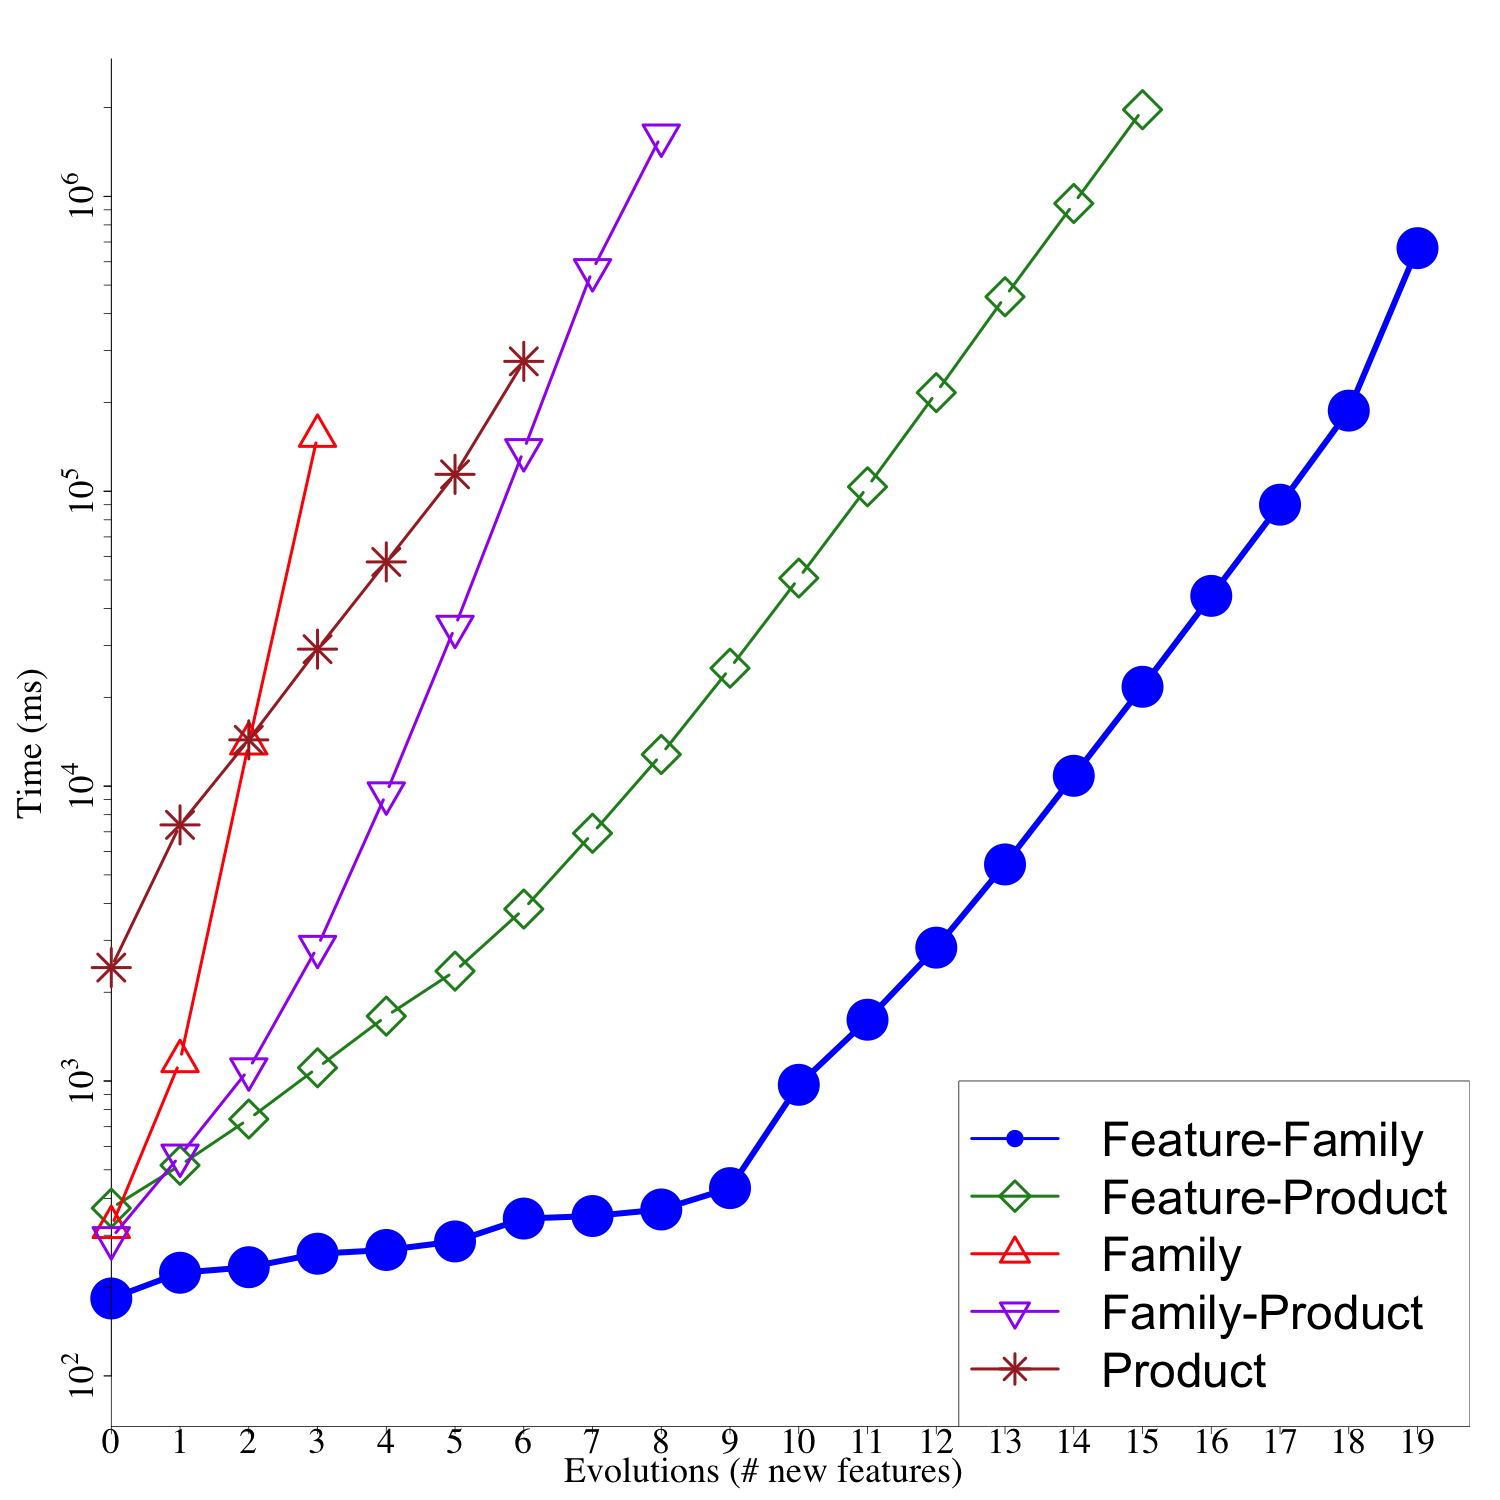
\includegraphics[width=1.0\columnwidth]{img/logemailTime}
    \caption{Analysis time.}
    \label{fig:email-analysisTime}
  \end{subfigure}
  \begin{subfigure}[t]{0.5\columnwidth}
    \centering
    %\includegraphics[width=1.0\columnwidth]{images/email-mean-memory-configurations_ascending-ALL}
    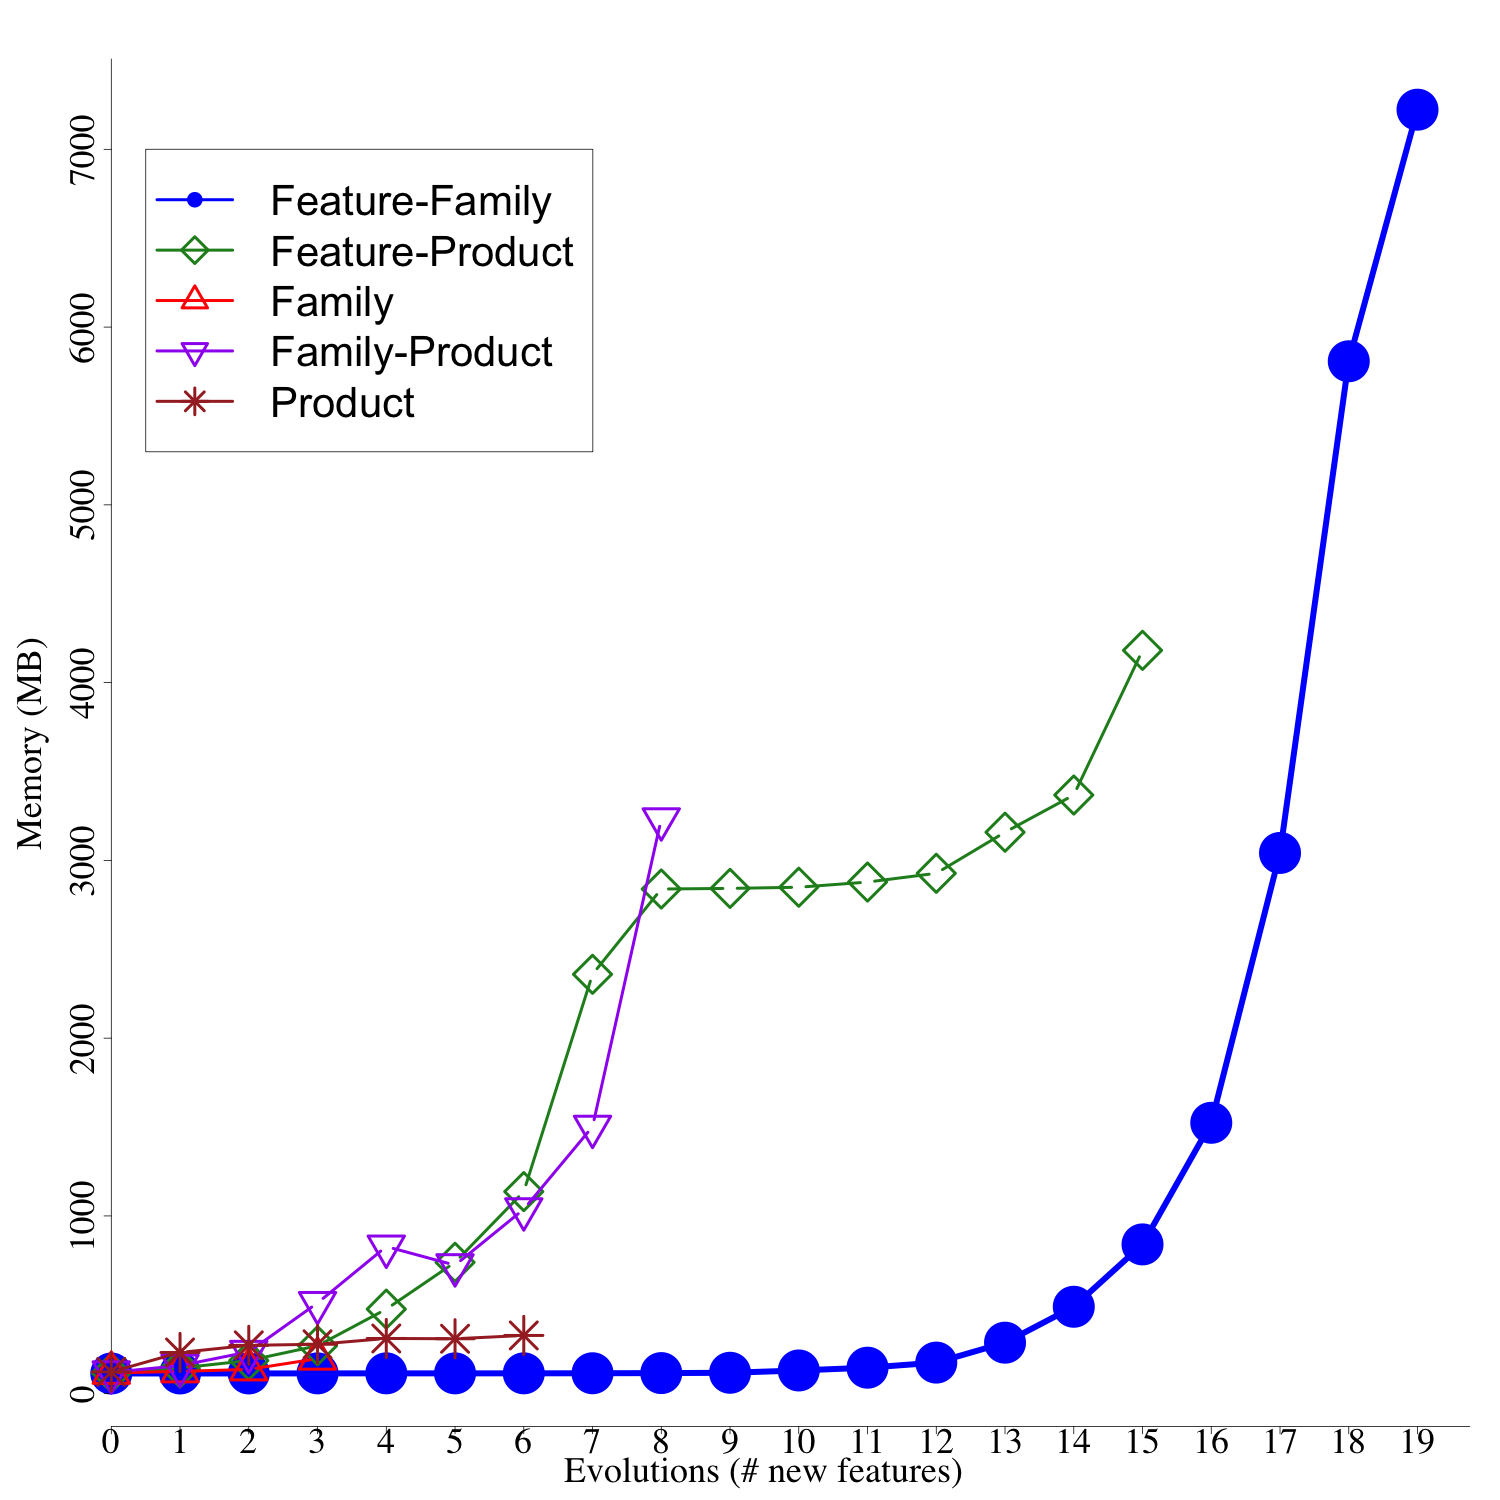
\includegraphics[width=1.0\columnwidth]{img/emailSpace}
    \caption{Demanded memory.}
    \label{fig:email-footprint}
  \end{subfigure}
  \caption{Time and memory required by different analysis strategies when
  evaluating evolutions of Email System.}
  \label{fig:email-scalability}
\end{figure}


\begin{figure}[p]
  \begin{subfigure}[t]{0.5\columnwidth}
    \centering
%    \includegraphics[width=1.0\columnwidth]{images/minepump-mean-analysis_time-configurations_ascending-logarithmic-ALL}
    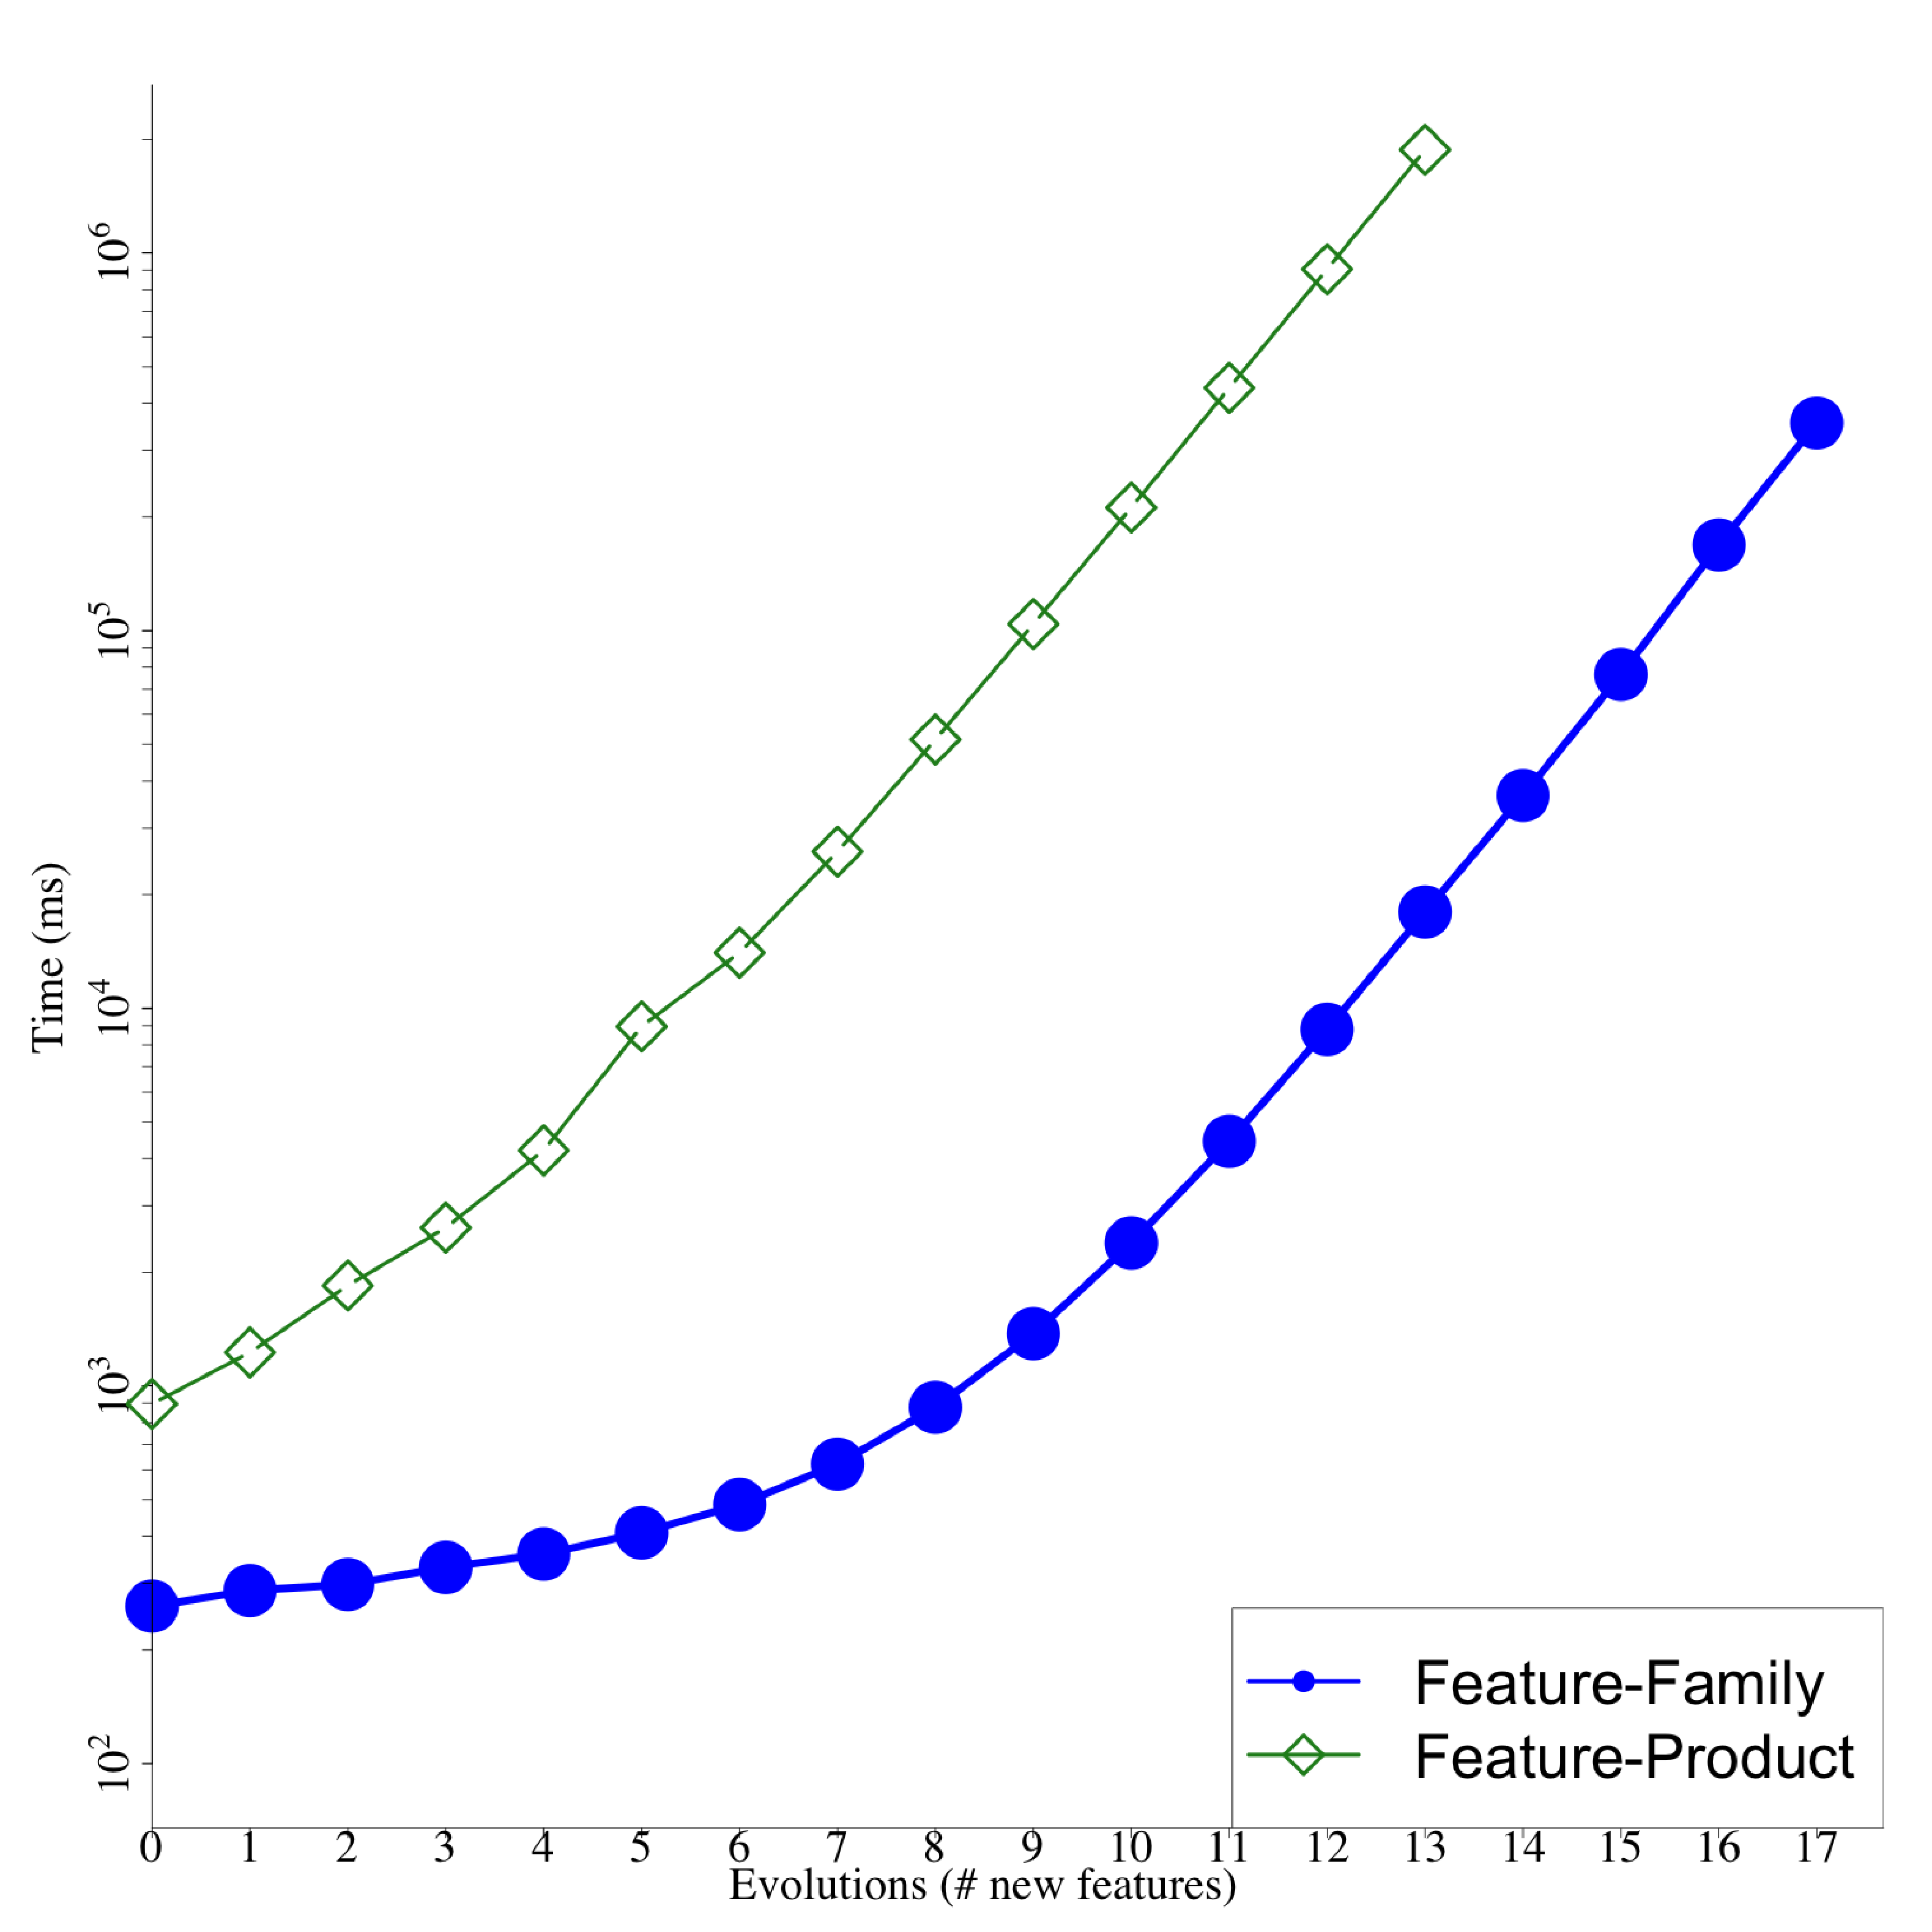
\includegraphics[width=1.0\columnwidth]{img/logminepumpTime}
    \caption{Analysis time.}
    \label{fig:minepump-analysisTime}
  \end{subfigure}
  \begin{subfigure}[t]{0.5\columnwidth}
    \centering
    %\includegraphics[width=1.0\columnwidth]{images/minepump-mean-memory-configurations_ascending-ALL}
    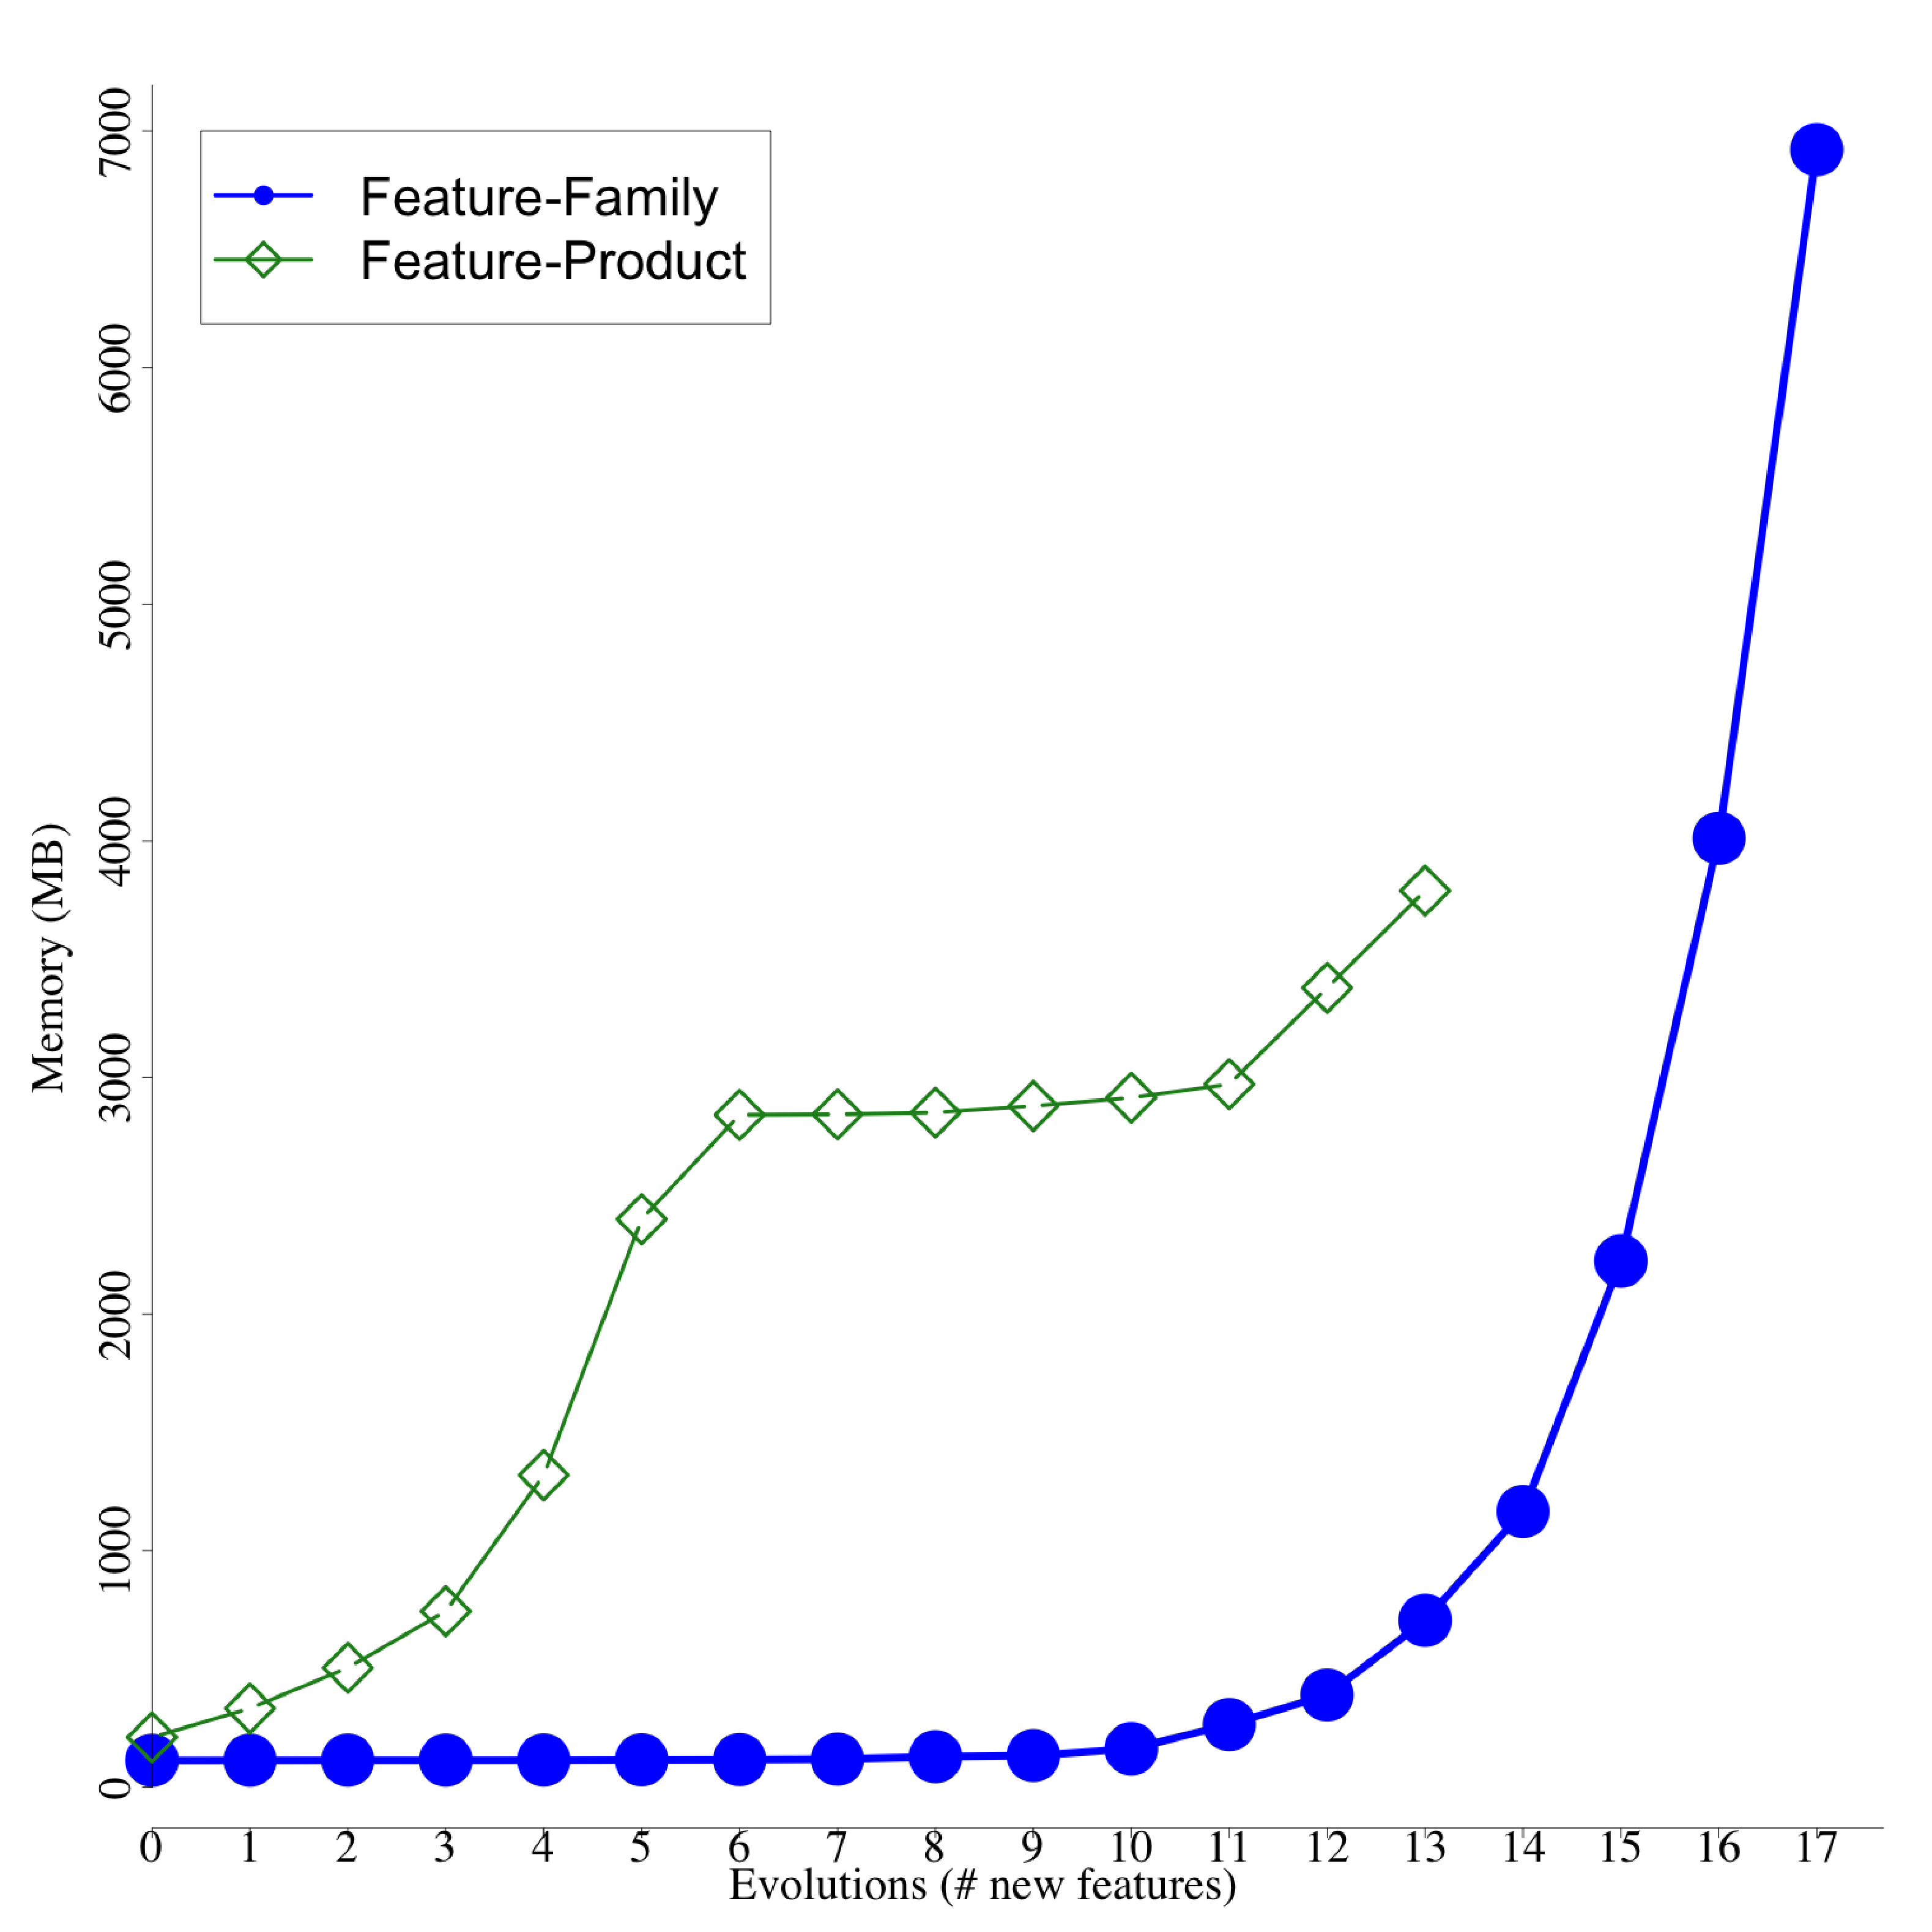
\includegraphics[width=1.0\columnwidth]{img/minepumpSpace}
    \caption{Demanded memory.}
    \label{fig:minepump-footprint}
  \end{subfigure}
  \caption{Time and memory required by different analysis strategies when
  evaluating evolutions of MinePump System.}
  \label{fig:minepump-scalability}
\end{figure}


\begin{figure}[p]
  \begin{subfigure}[t]{0.5\columnwidth}
    \centering
%    \includegraphics[width=1.0\columnwidth]{images/bsn-mean-analysis_time-configurations_ascending-logarithmic-ALL}
    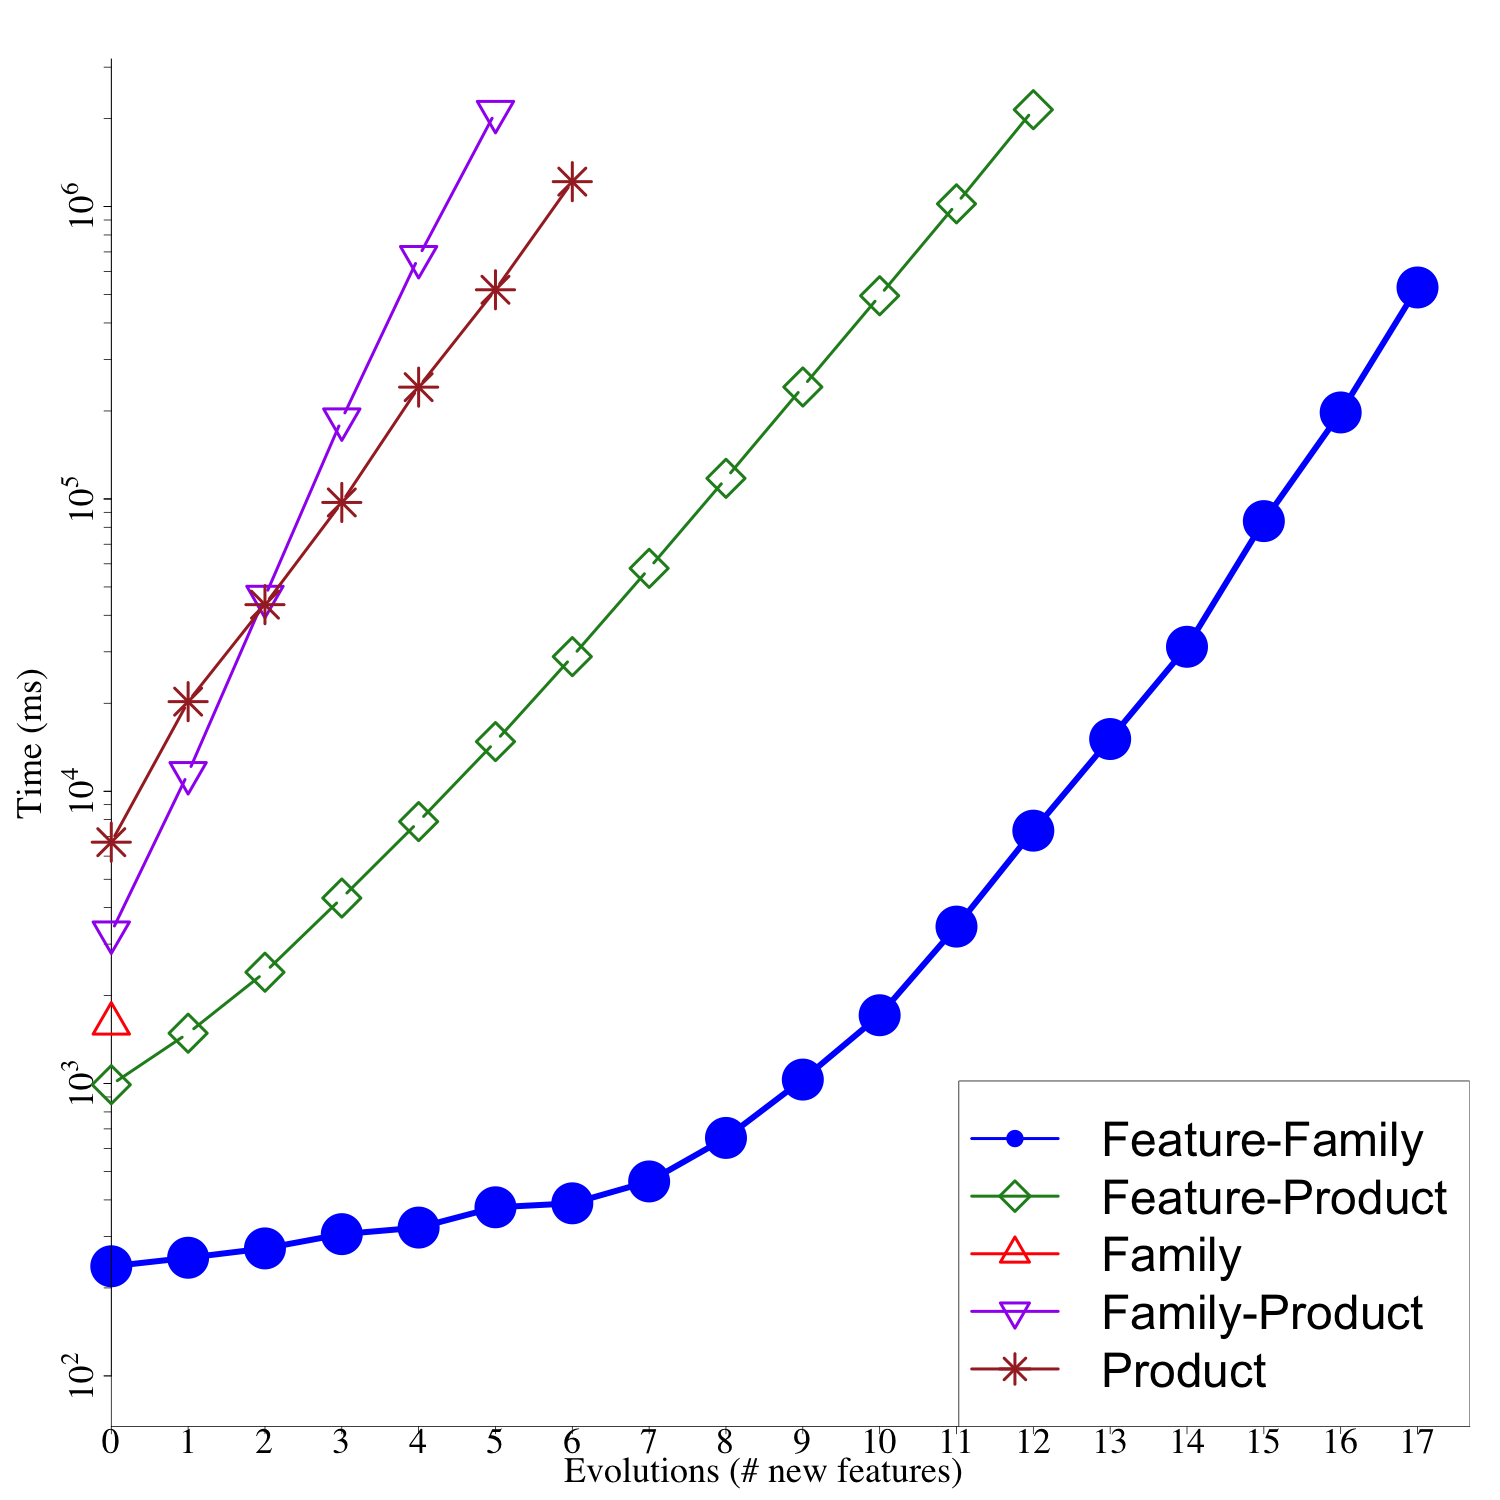
\includegraphics[width=1.0\columnwidth]{img/logbsnTime}
    \caption{Analysis time.}
    \label{fig:bsn-analysisTime}
  \end{subfigure}
  \begin{subfigure}[t]{0.5\columnwidth}
    \centering
    %\includegraphics[width=1.0\columnwidth]{images/bsn-mean-memory-configurations_ascending-ALL}
    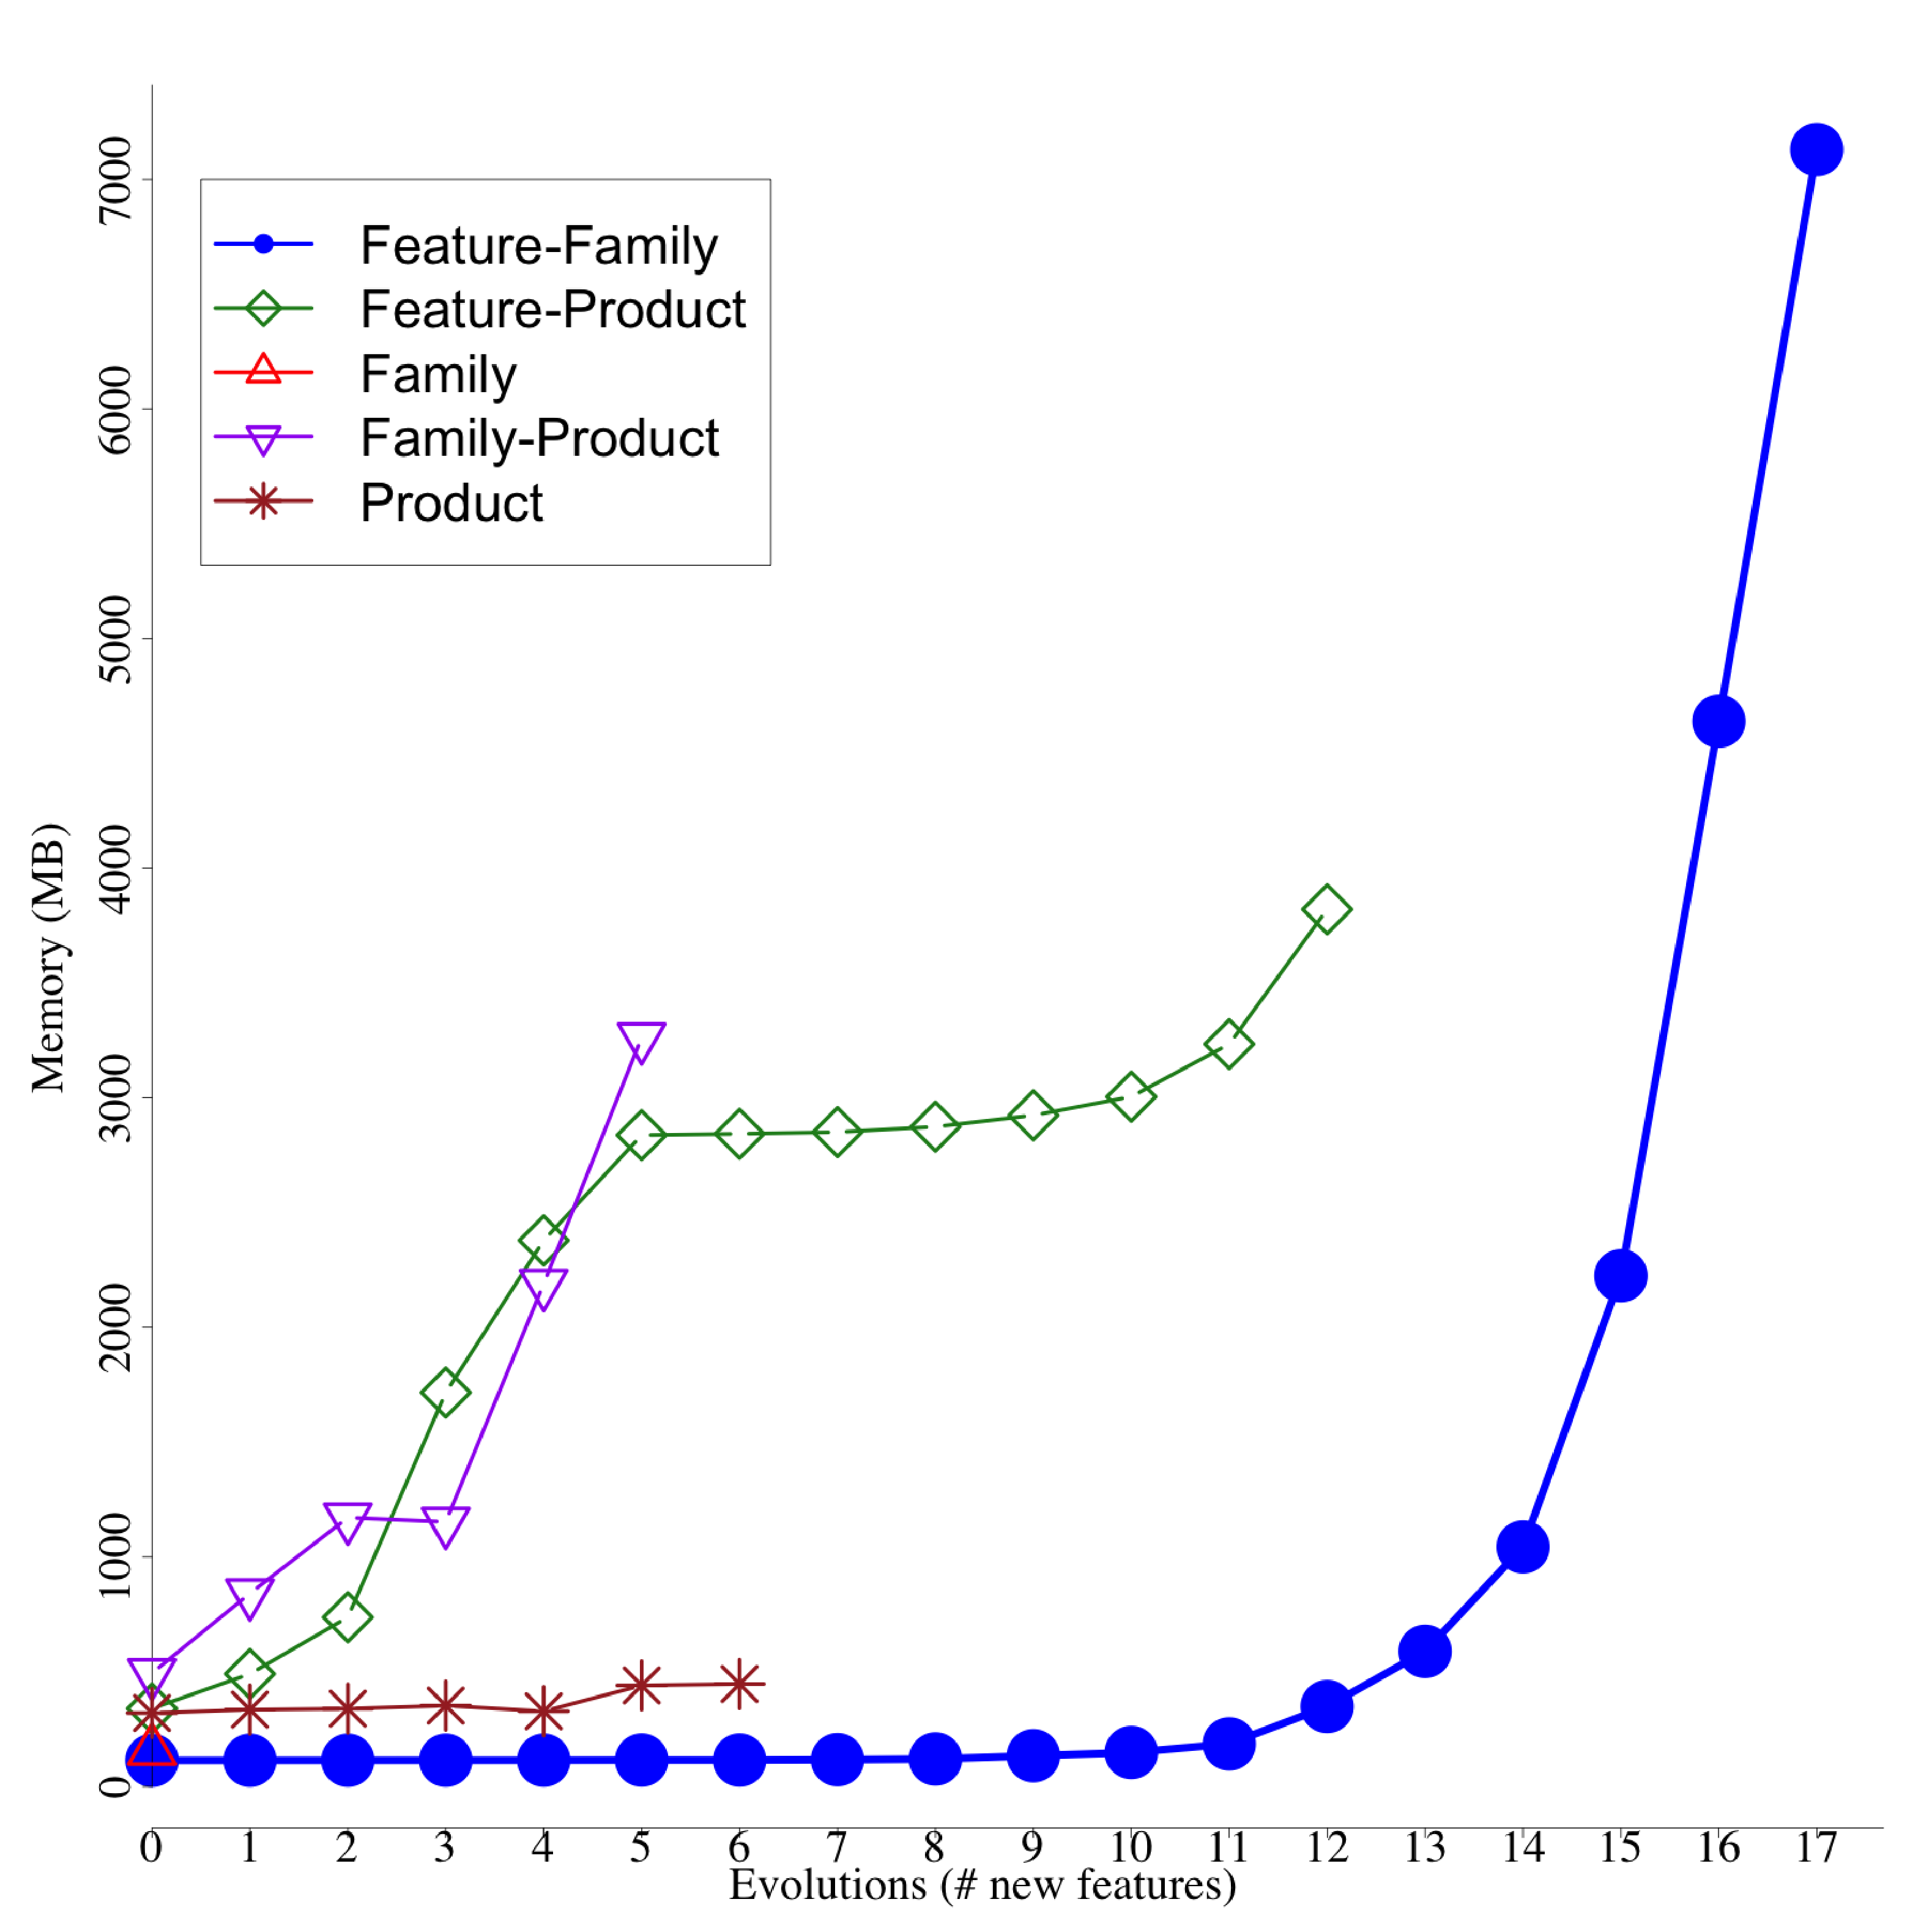
\includegraphics[width=1.0\columnwidth]{img/bsnSpace}
    \caption{Demanded memory.}
    \label{fig:bsn-footprint}
  \end{subfigure}
  \caption{Time and memory required by different analysis strategies when
  evaluating evolutions of BSN-SPL.}
  \label{fig:bsn-scalability}
\end{figure}


\begin{figure}[p]
  \begin{subfigure}[t]{0.5\columnwidth}
    \centering
%    \includegraphics[width=1.0\columnwidth]{images/lift-mean-analysis_time-configurations_ascending-logarithmic-ALL}
    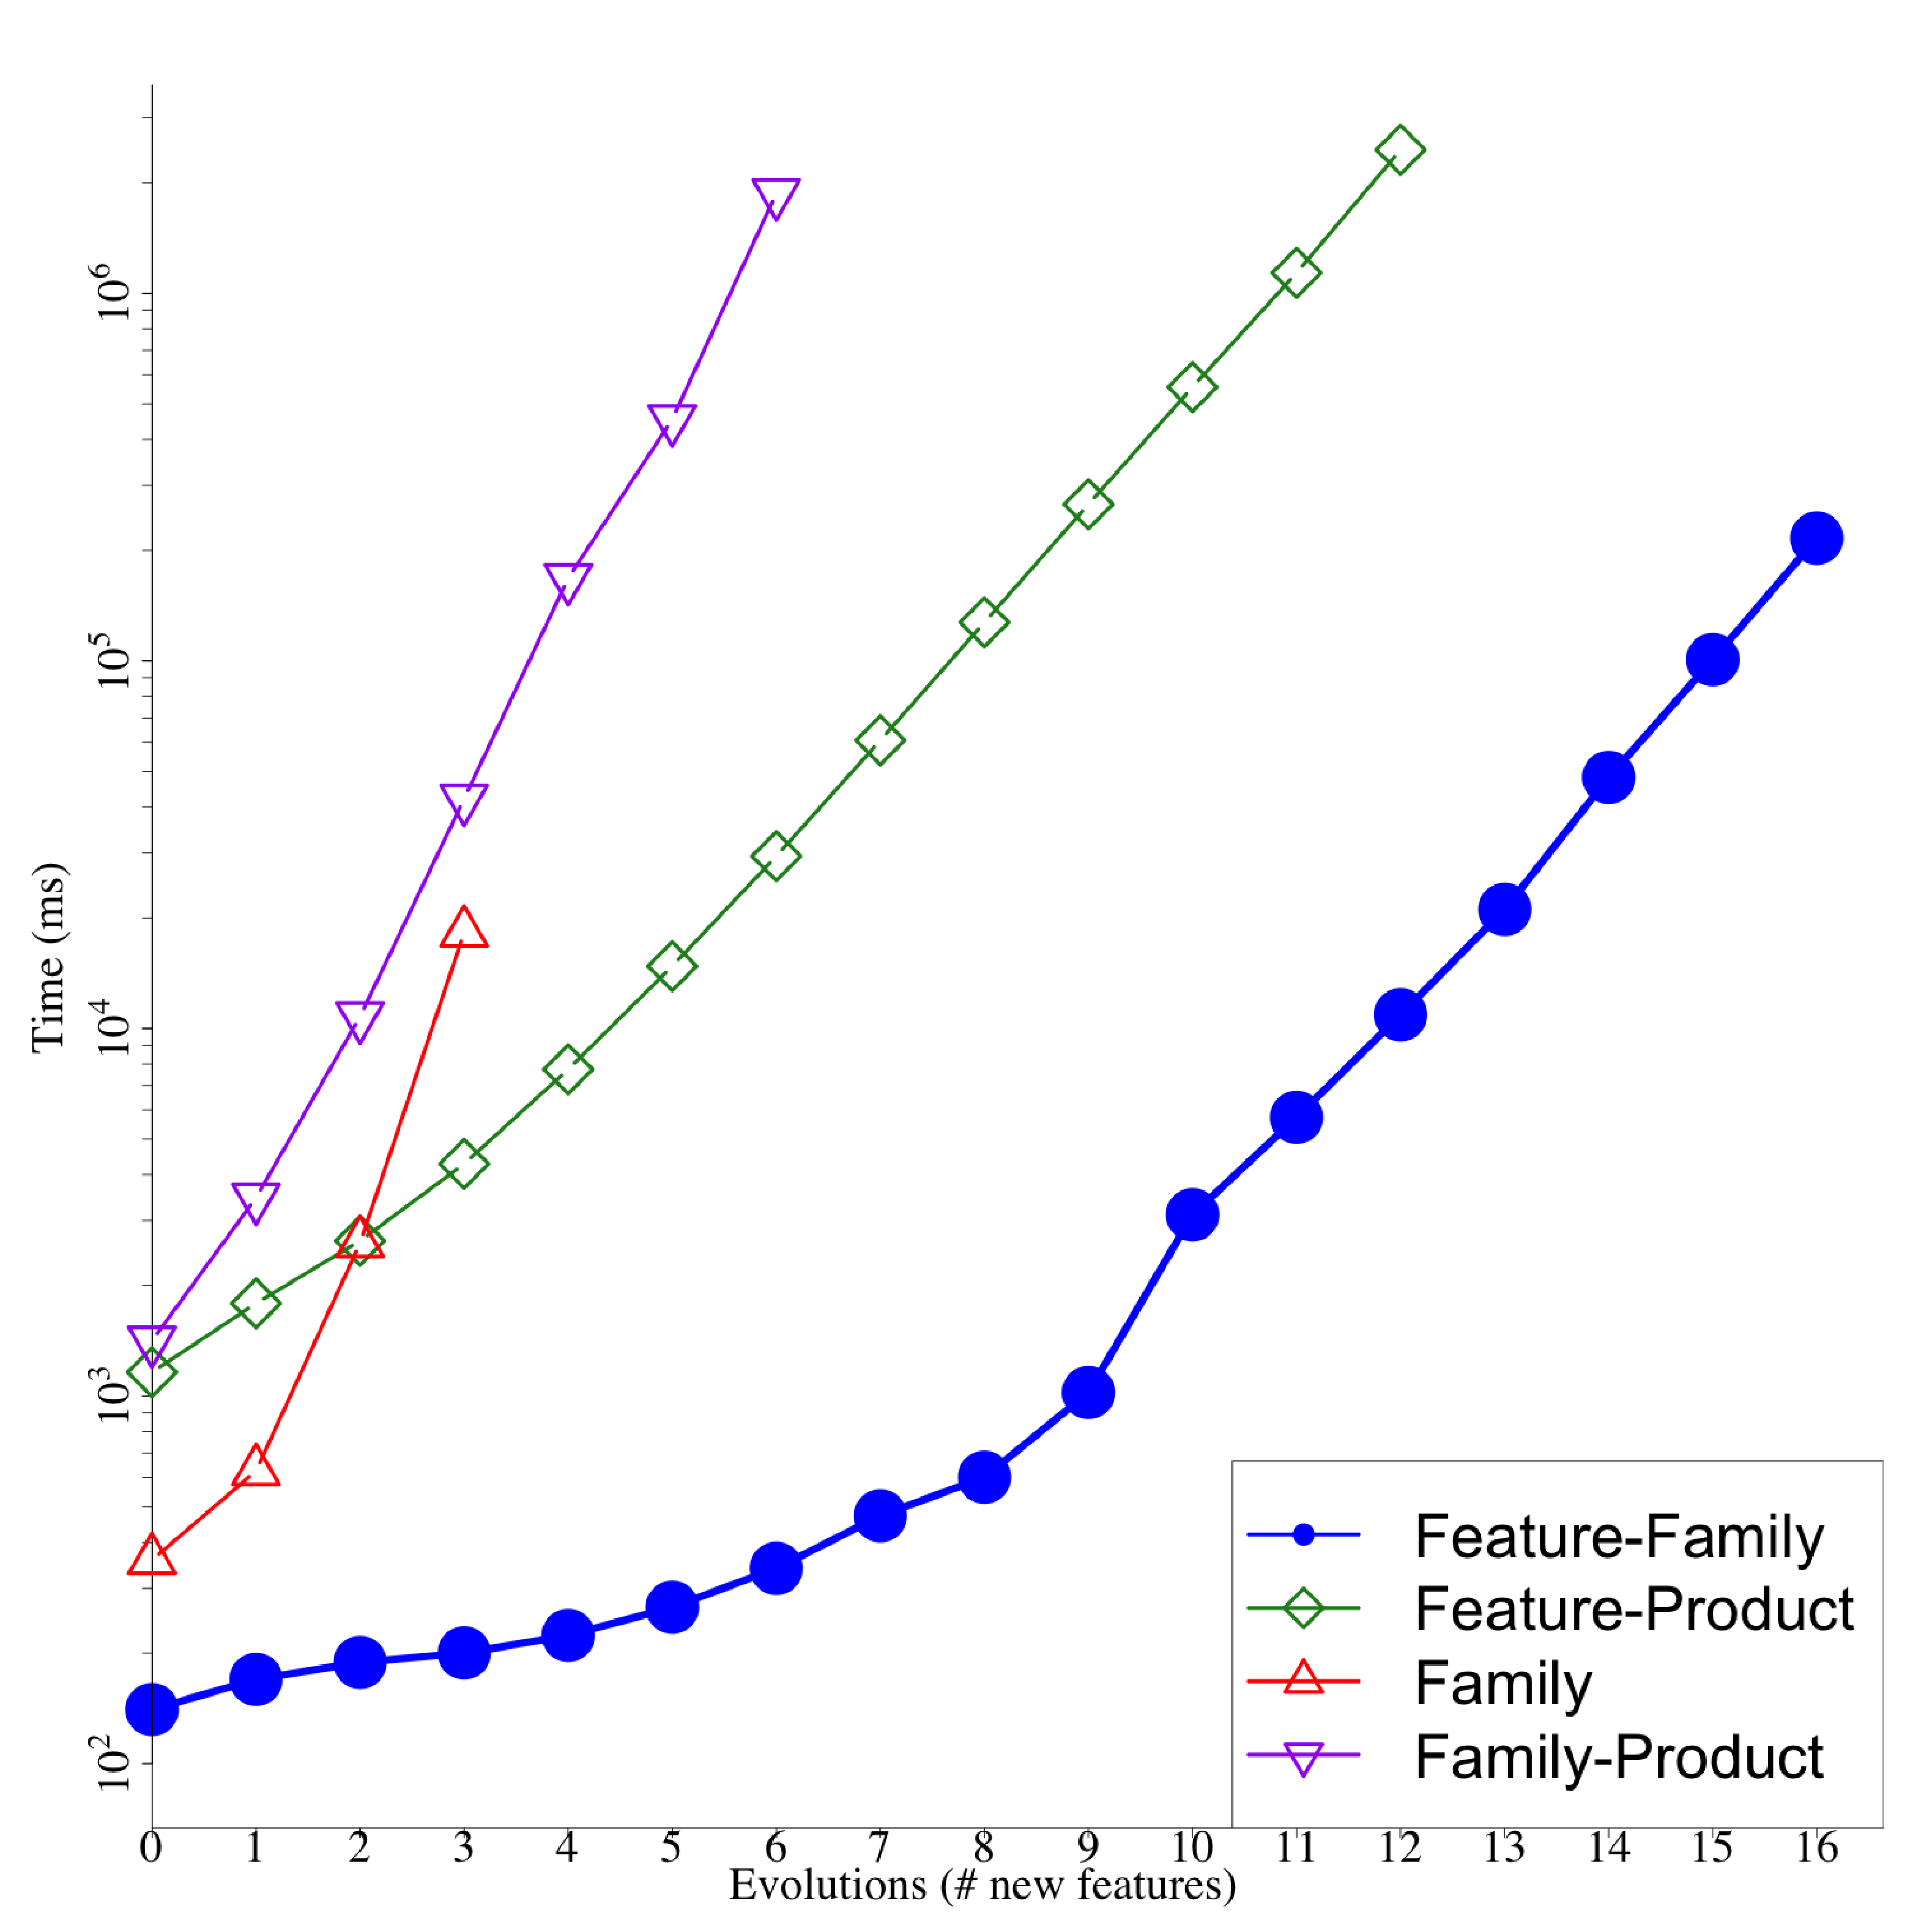
\includegraphics[width=1.0\columnwidth]{img/logliftTime}
    \caption{Analysis time.}
    \label{fig:lift-analysisTime}
  \end{subfigure}
  \begin{subfigure}[t]{0.5\columnwidth}
    \centering
    %\includegraphics[width=1.0\columnwidth]{images/lift-mean-memory-configurations_ascending-ALL}
    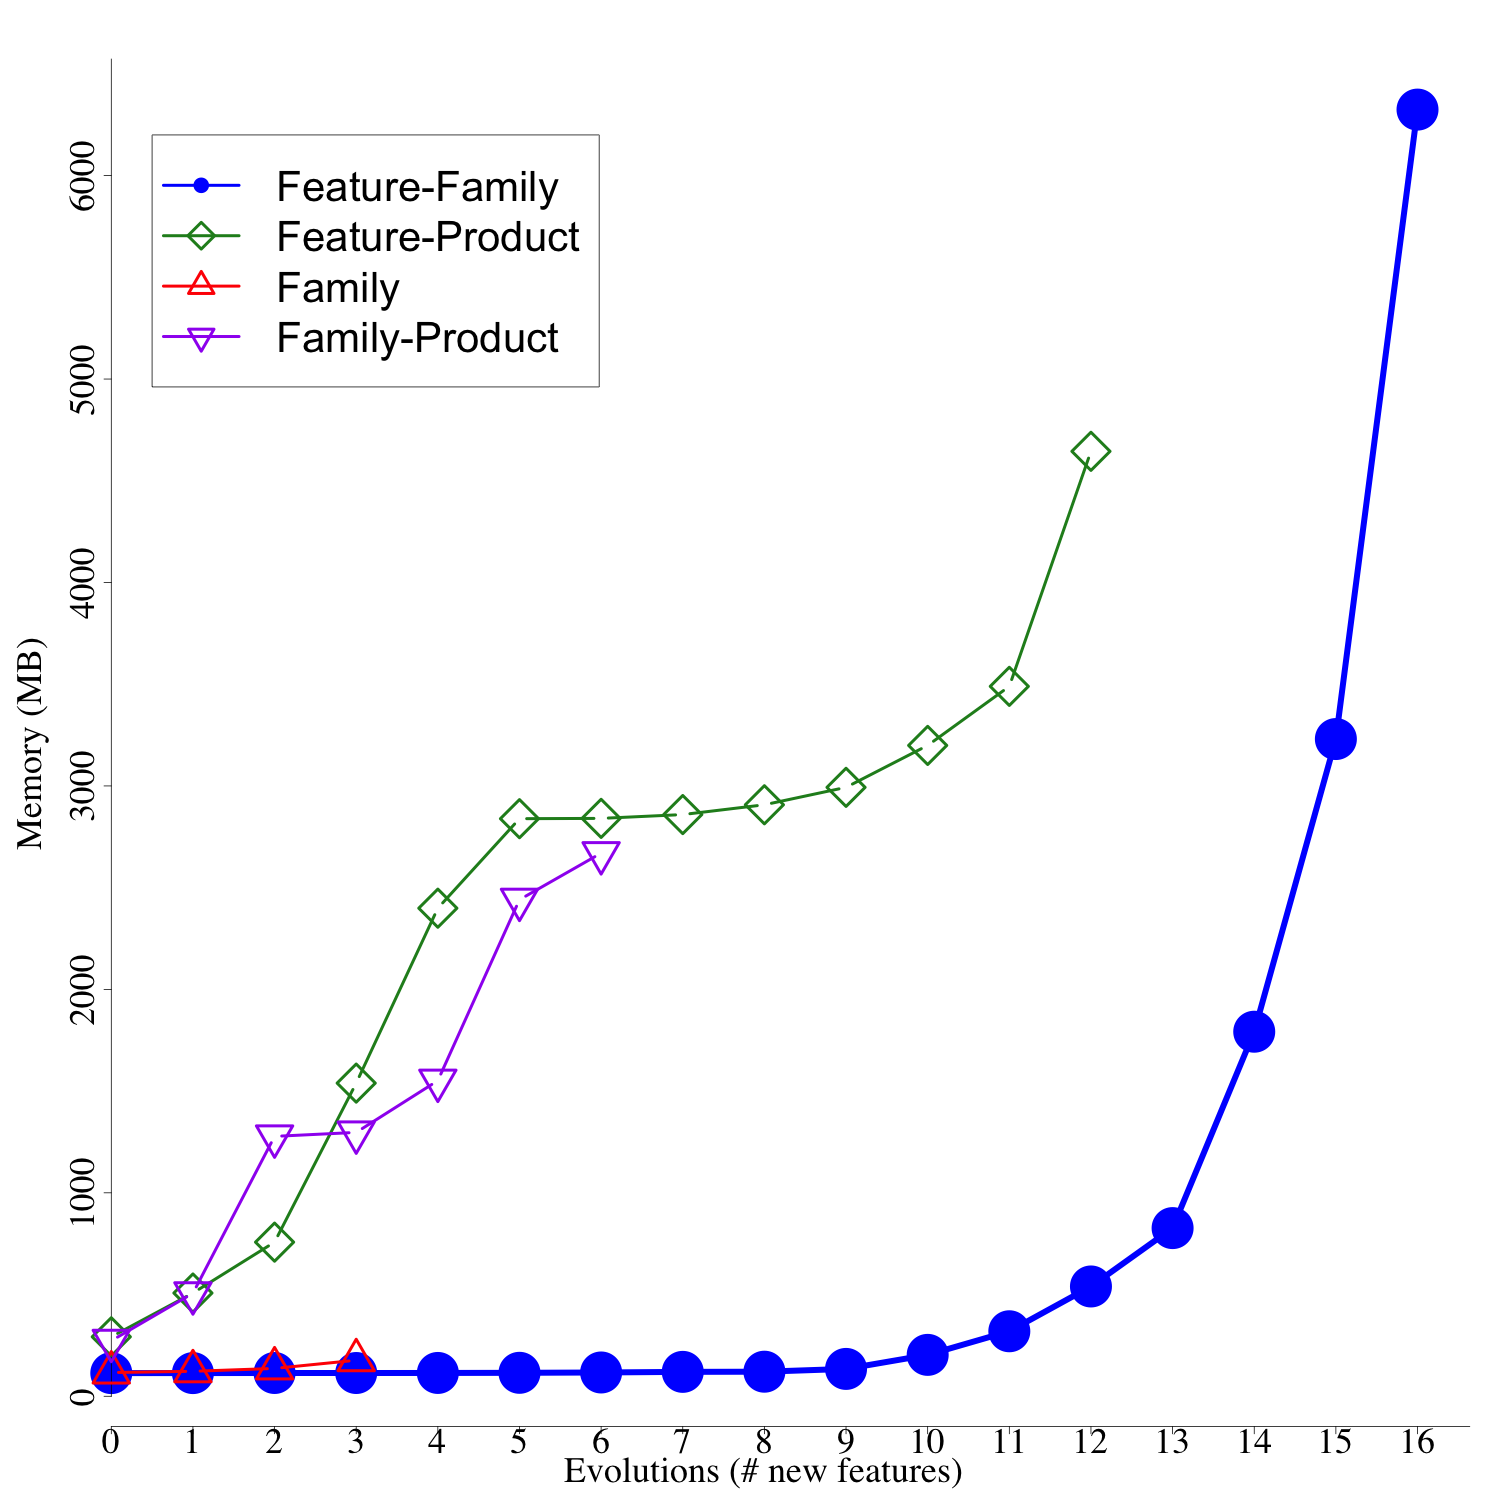
\includegraphics[width=1.0\columnwidth]{img/liftSpace}
    \caption{Demanded memory.}
    \label{fig:lift-footprint}
  \end{subfigure}
  \caption{Time and memory required by different analysis strategies when
  evaluating evolutions of Lift System.}
  \label{fig:lift-scalability}
\end{figure}


\begin{figure}[p]
  \begin{subfigure}[t]{0.5\columnwidth}
    \centering
%    \includegraphics[width=1.0\columnwidth]{images/intercloud-mean-analysis_time-configurations_ascending-logarithmic-ALL}
    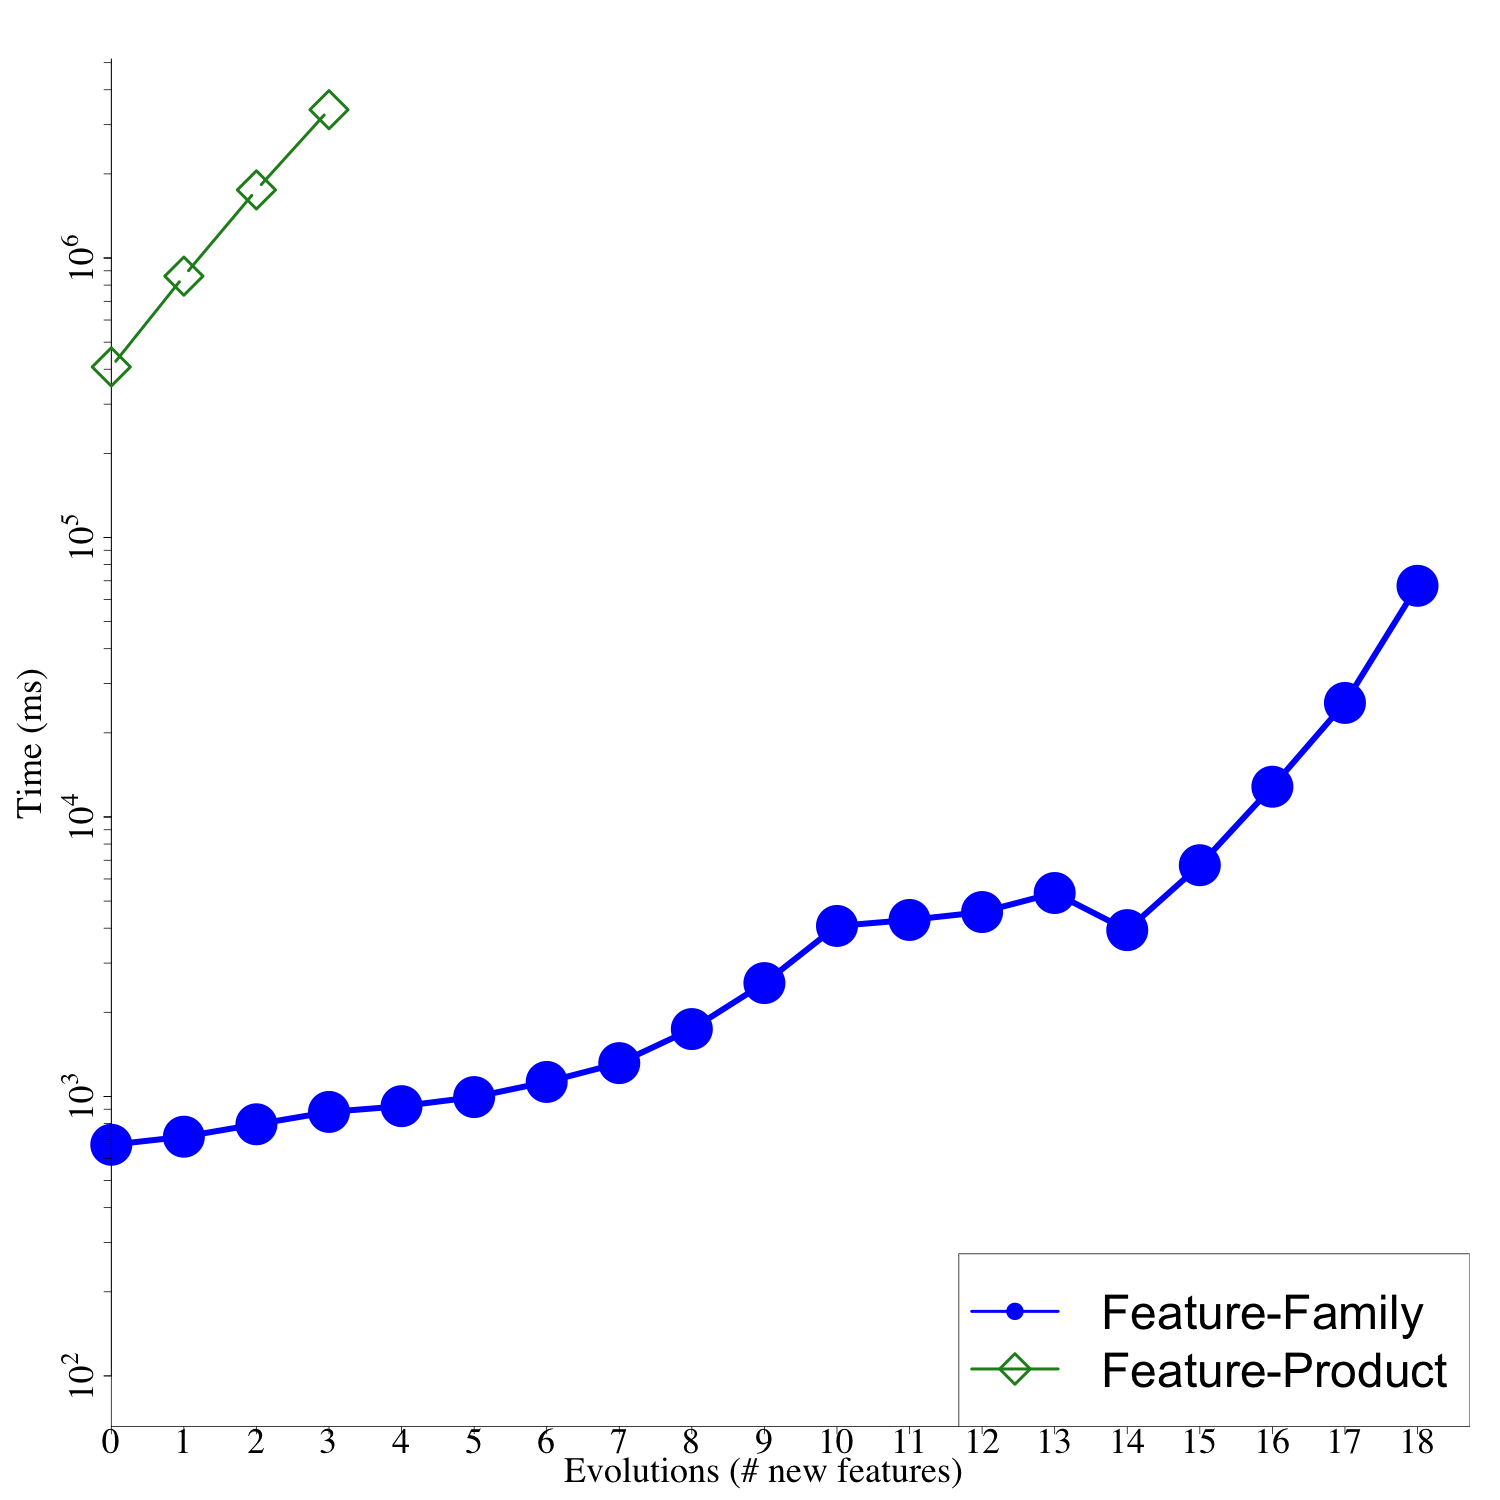
\includegraphics[width=1.0\columnwidth]{img/logintercloudTime}
    \caption{Analysis time.}
    \label{fig:intercloud-analysisTime}
  \end{subfigure}
  \begin{subfigure}[t]{0.5\columnwidth}
    \centering
    %\includegraphics[width=1.0\columnwidth]{images/intercloud-mean-memory-configurations_ascending-ALL}
    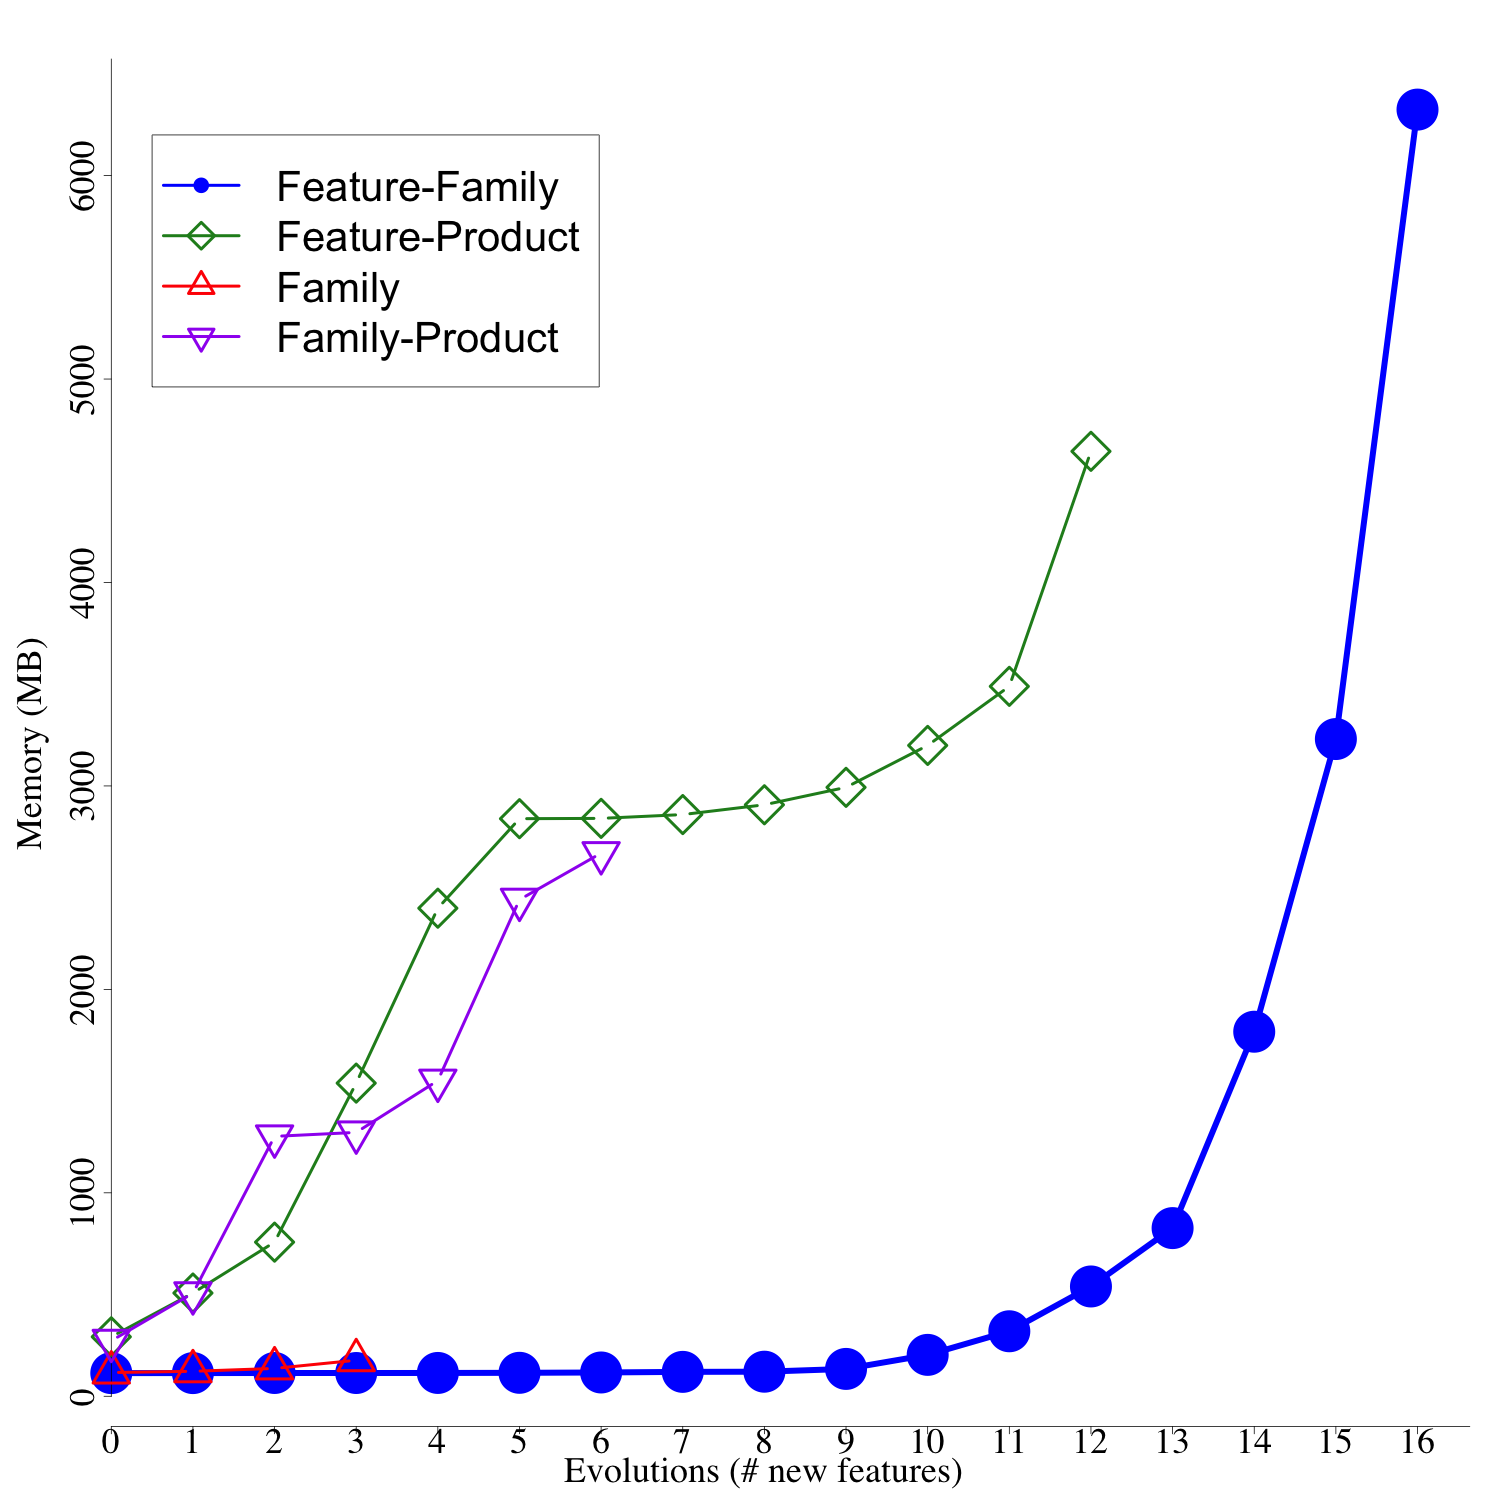
\includegraphics[width=1.0\columnwidth]{img/intercloudSpace}
    \caption{Demanded memory.}
    \label{fig:intercloud-footprint}
  \end{subfigure}
  \caption{Time and memory required by different analysis strategies when
  evaluating evolutions of InterCloud System.}
  \label{fig:intercloud-scalability}
\end{figure}


\begin{figure}[p]
  \begin{subfigure}[t]{0.5\columnwidth}
    \centering
%    \includegraphics[width=1.0\columnwidth]{images/tankwar-mean-analysis_time-configurations_ascending-logarithmic-ALL}
    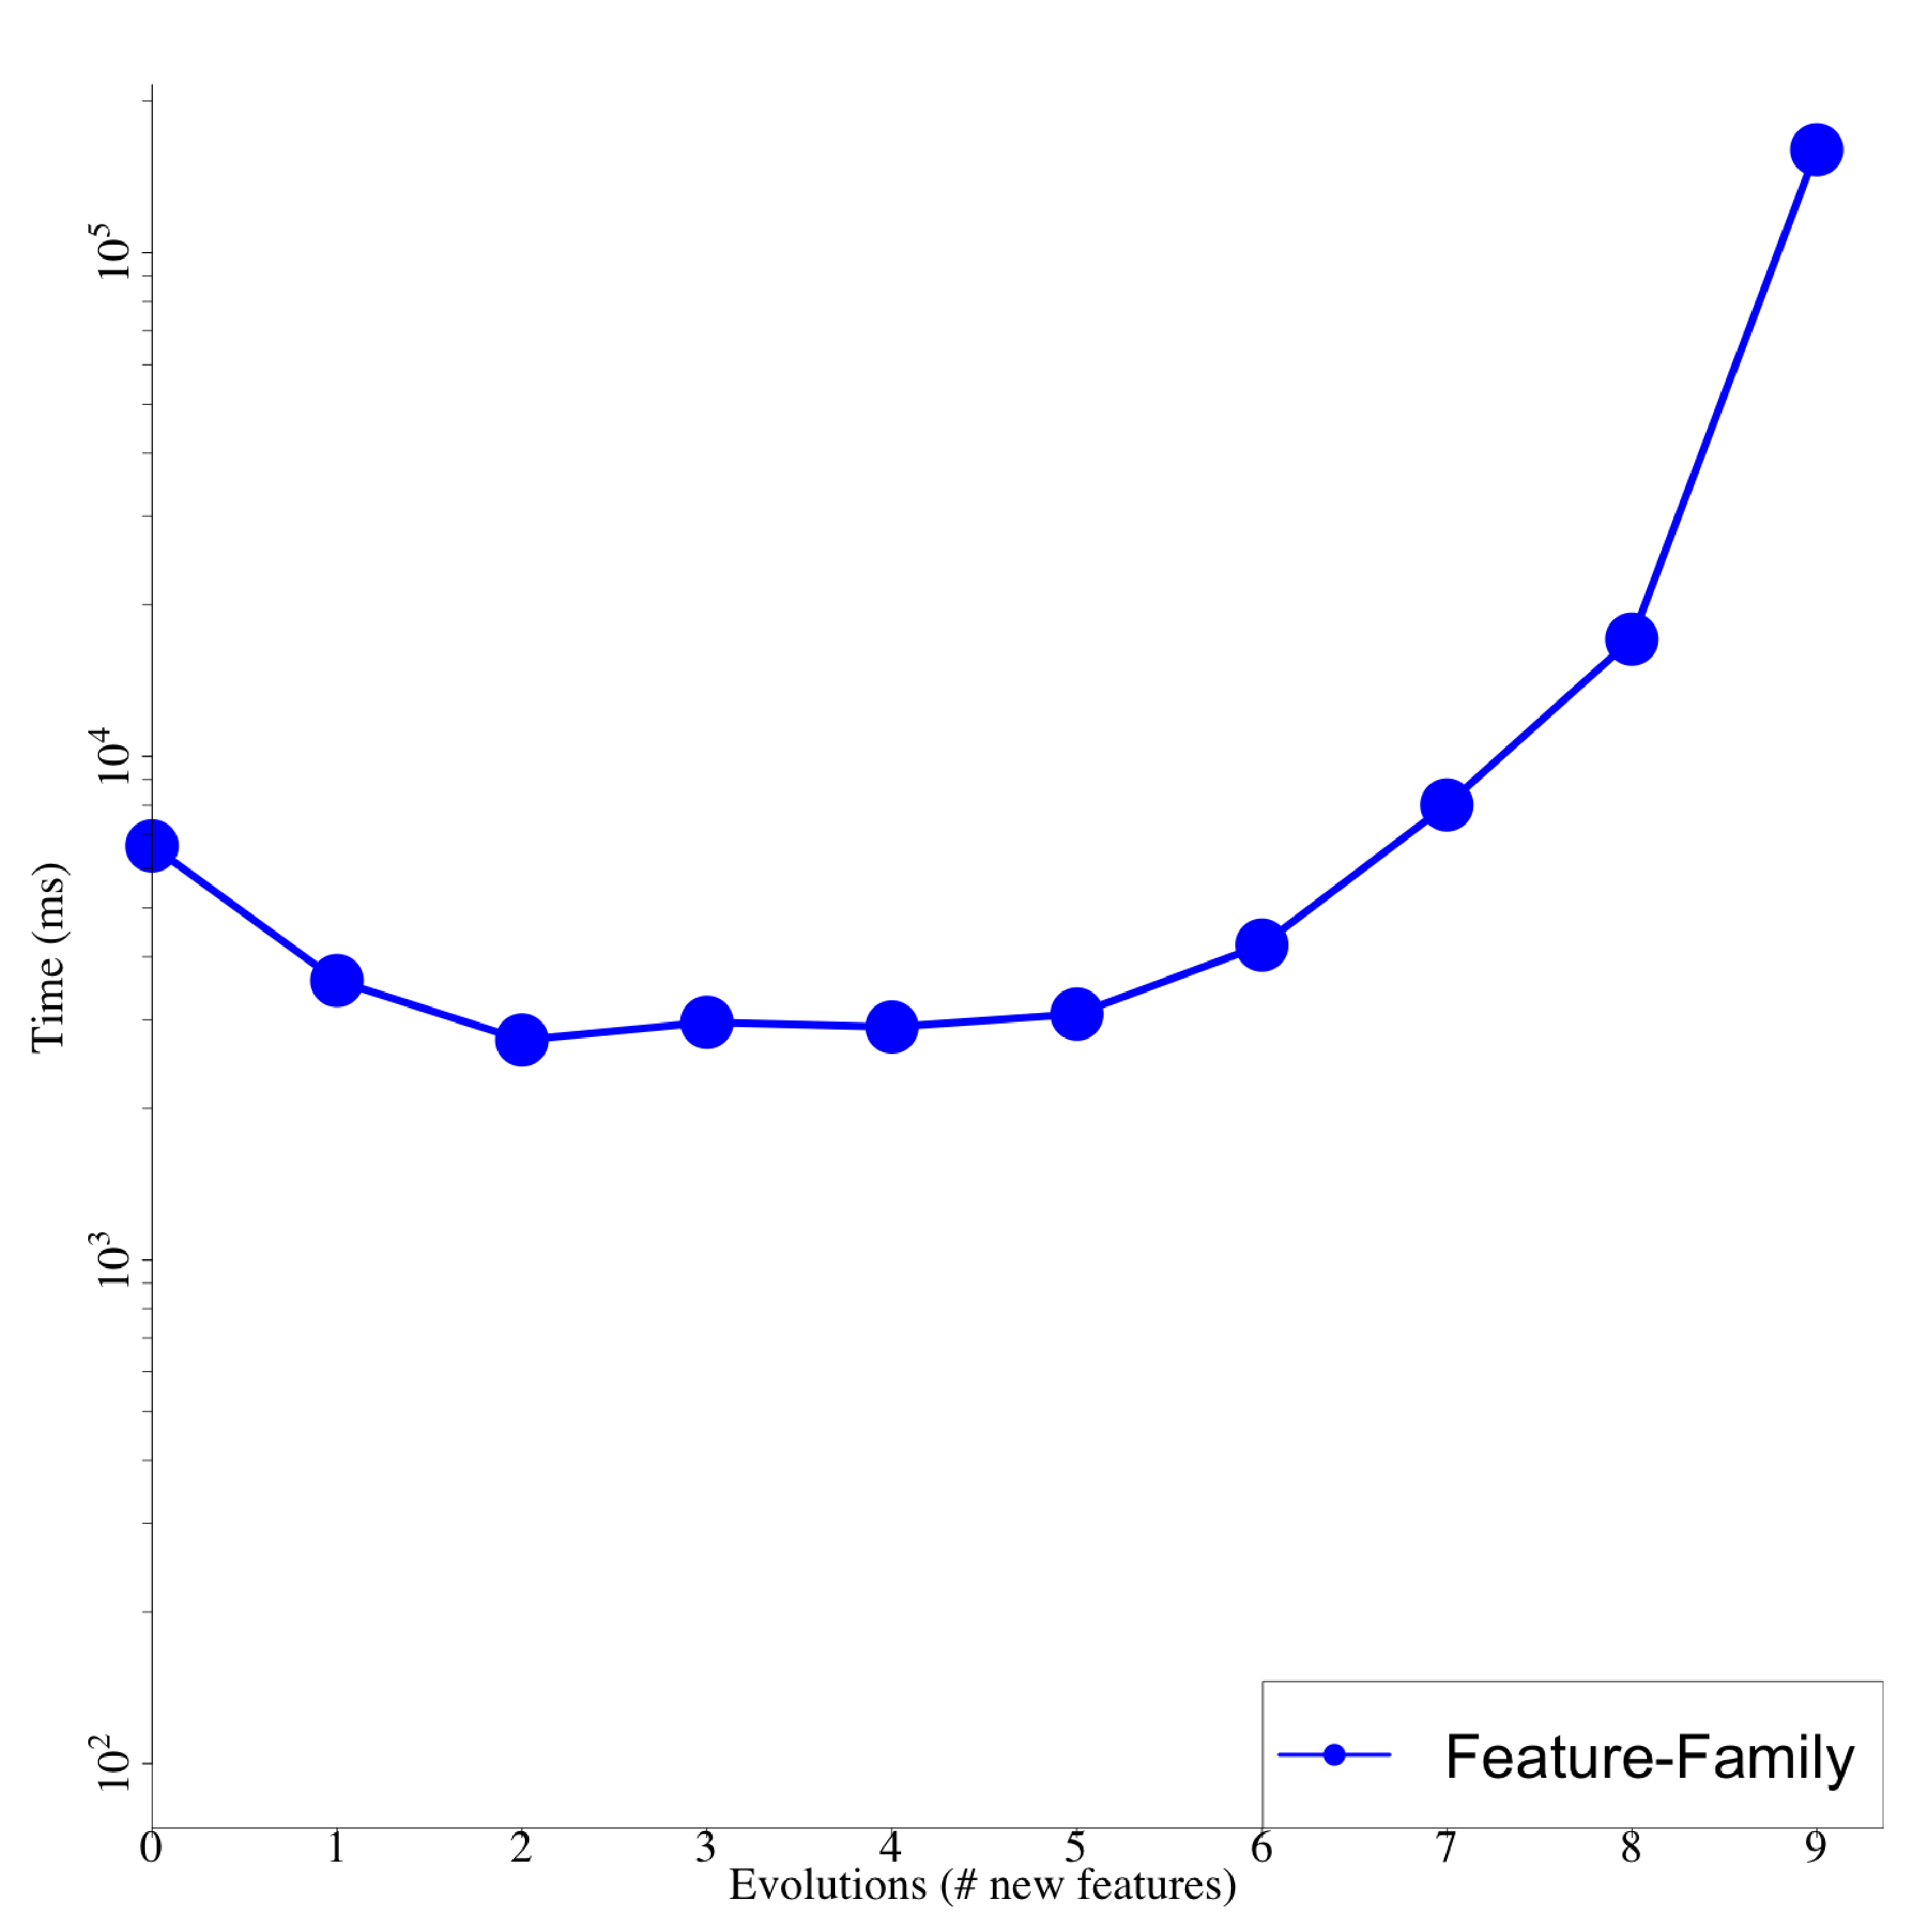
\includegraphics[width=1.0\columnwidth]{img/logtankwarTime}
    \caption{Analysis time.}
    \label{fig:tankwar-analysisTime}
  \end{subfigure}
  \begin{subfigure}[t]{0.5\columnwidth}
    \centering
    %\includegraphics[width=1.0\columnwidth]{images/tankwar-mean-memory-configurations_ascending-ALL}
    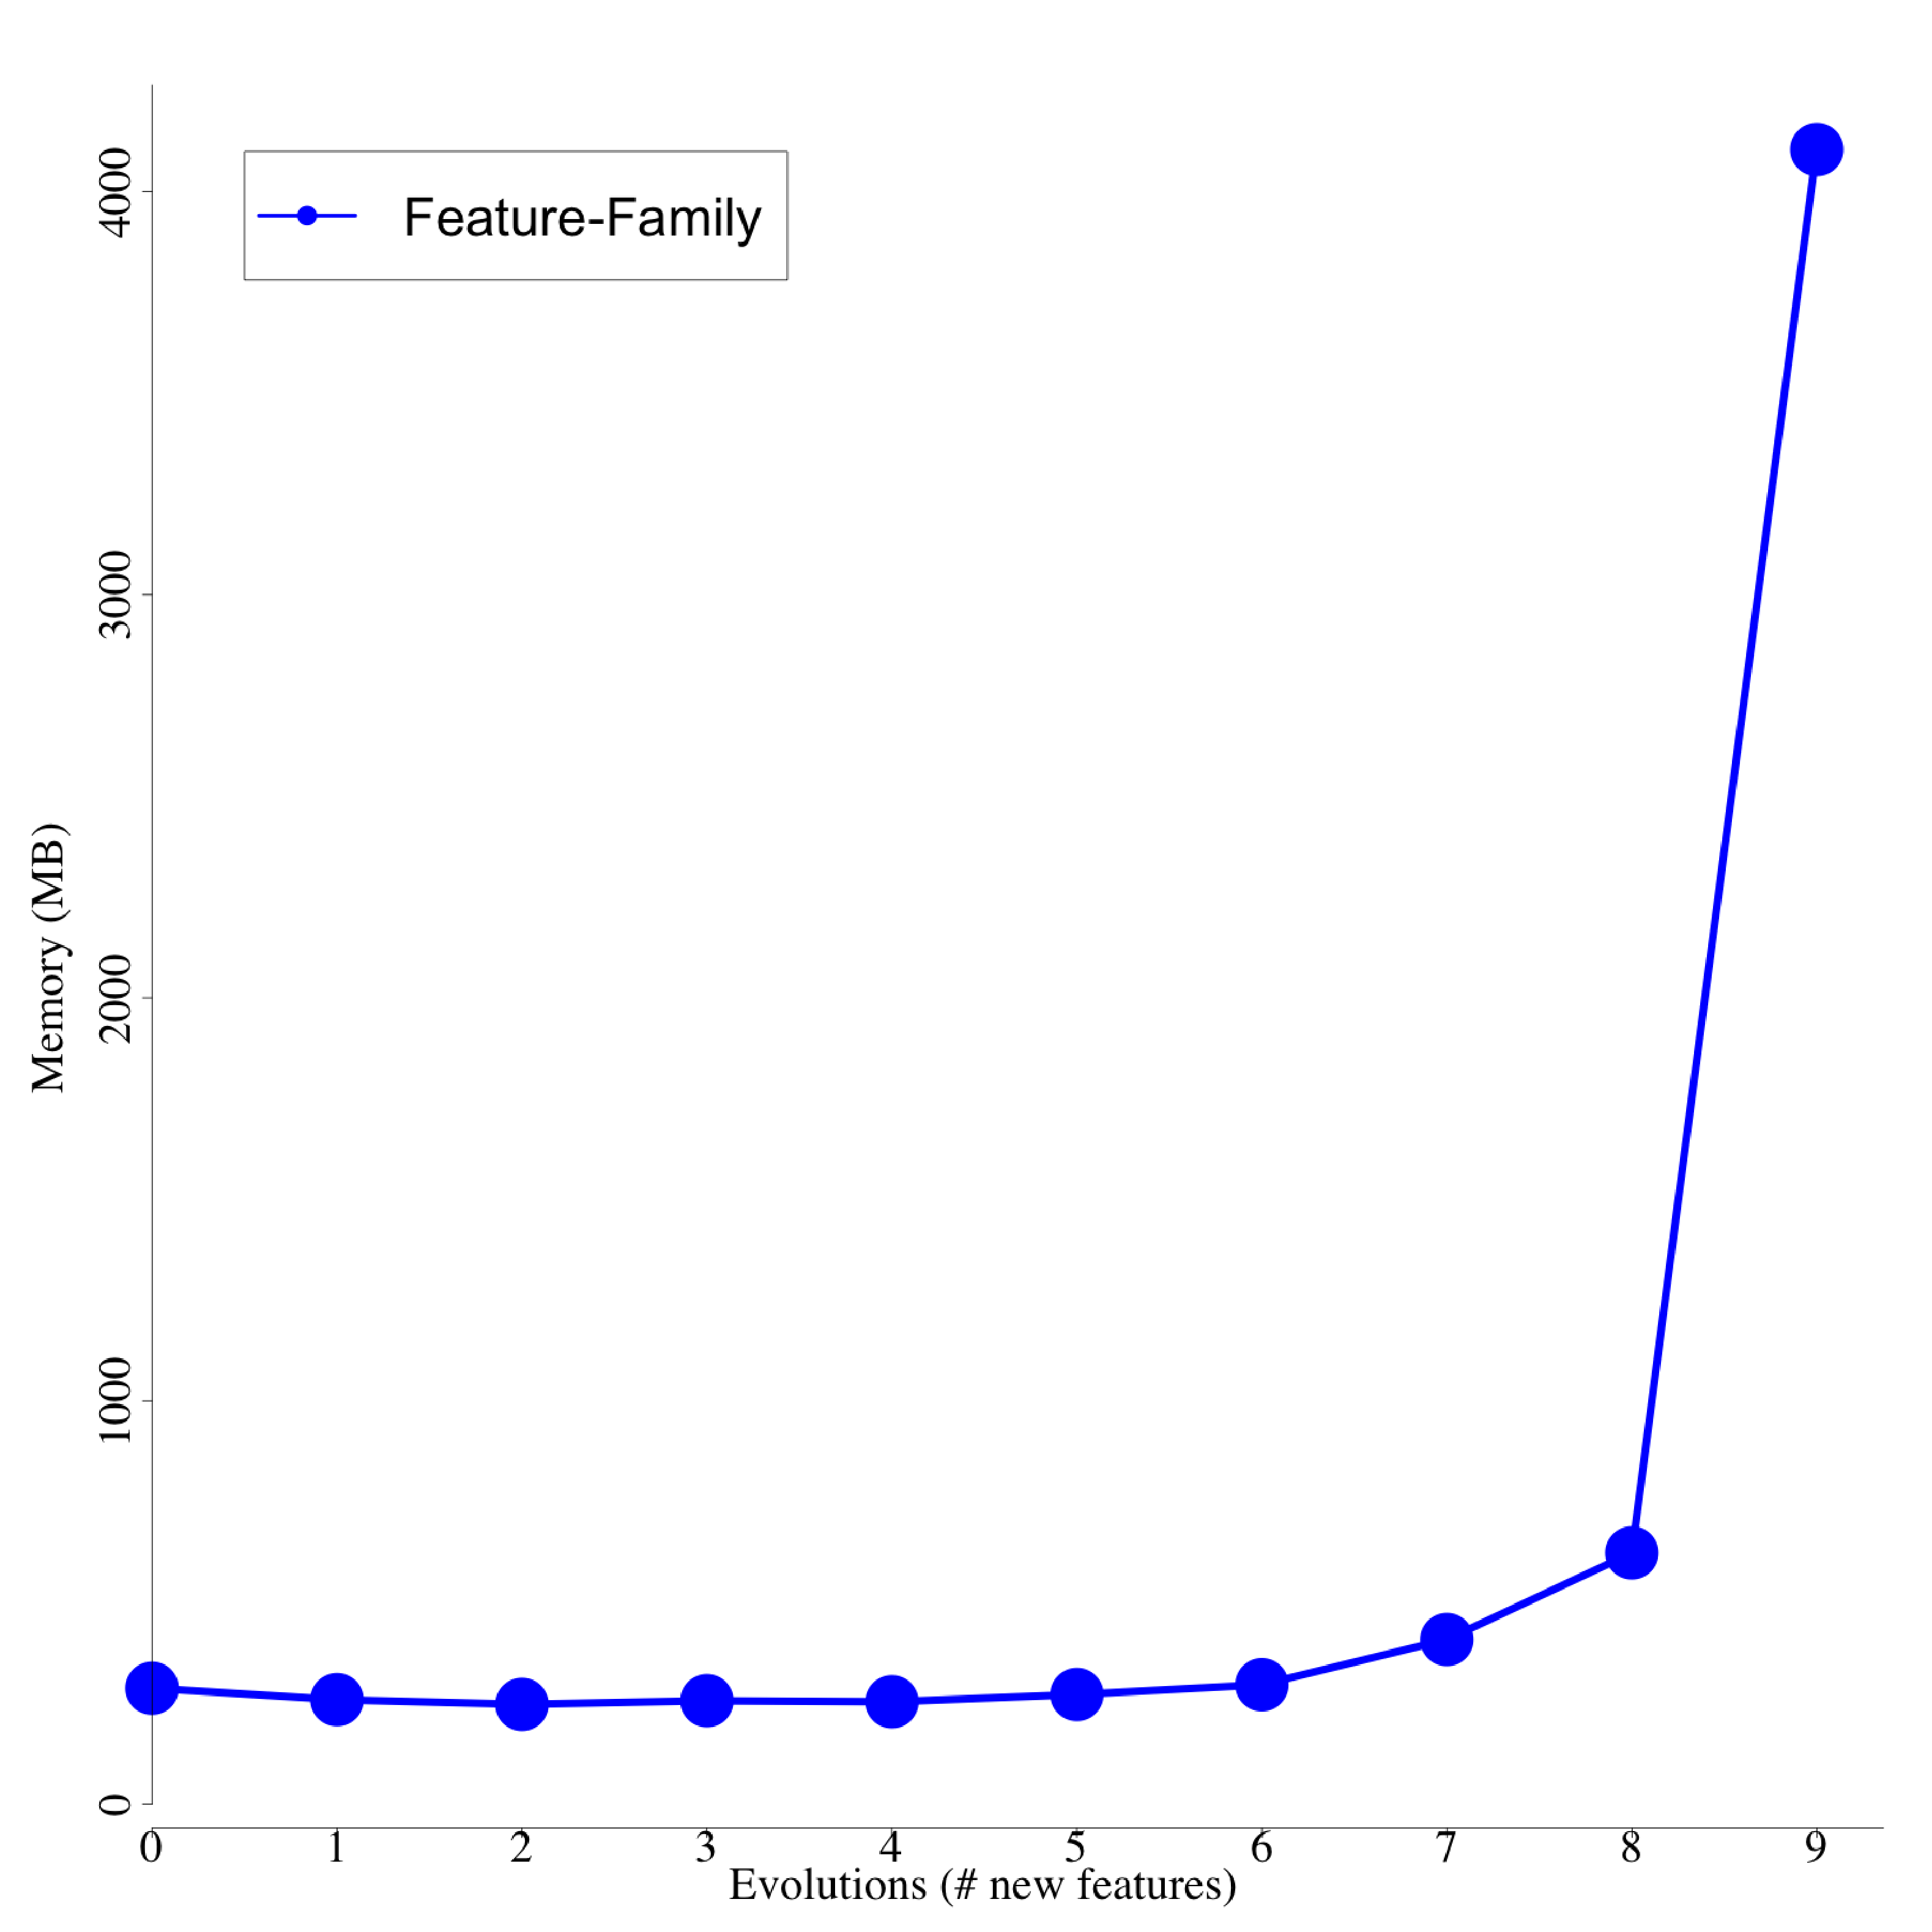
\includegraphics[width=1.0\columnwidth]{img/tankwarSpace}
    \caption{Demanded memory.}
    \label{fig:tankwar-footprint}
  \end{subfigure}
  \caption{Time and memory required by different analysis strategies when
  evaluating evolutions of TankWar battle game.}
  \label{fig:tankwar-scalability}
\end{figure}


Overall, the experiments show with statistical significance that the
feature-family-based strategy is faster than all other analysis strategies (as
shown in Figures \ref{fig:email-analysisTime}, \ref{fig:minepump-analysisTime},
\ref{fig:bsn-analysisTime}, \ref{fig:lift-analysisTime},
\ref{fig:intercloud-analysisTime}, and \ref{fig:tankwar-analysisTime}).
Regarding execution time, in the worst case, the feature-family-based strategy
performed $60\%$ faster than the family-product-based strategy, when analyzing
the original models of the Email product line
(Figure~\ref{fig:email-analysisTime}); in the best case, it outperformed the
family-product-based analysis of the BSN product line with $4$ optional features
added (i.e., its $5^{th}$ evolution step---Figure~\ref{fig:bsn-analysisTime}) by
4 orders of magnitude. Such cases are highlighted in yellow in
Table~A1.  Regarding memory consumption
(Figures~\ref{fig:email-footprint}, \ref{fig:minepump-footprint},
\ref{fig:bsn-footprint}, \ref{fig:lift-footprint},
\ref{fig:intercloud-footprint}, and \ref{fig:tankwar-footprint}), the experiment
also shows with statistical significance that,   in the worst case, the
feature-family-based strategy demanded $2\%$ less memory than the family-based
strategy when analyzing the original model of the Lift product line; in the best
case, it saved around 4,757 megabytes when analyzing the $3^{rd}$ evolution step
of the InterCloud product line. Such cases are highlighted in yellow in
Table~A2.

% Overall, our experiments show that the feature-family-based strategy is both
% faster and less memory-consuming, with statistical significance, than all
% other analysis strategies (as shown in Figures \ref{fig:email-analysisTime},
% \ref{fig:minepump-analysisTime}, \ref{fig:bsn-analysisTime},
% \ref{fig:lift-analysisTime}, \ref{fig:intercloud-analysisTime}, and
% \ref{fig:tankwar-analysisTime}). Regarding execution time, in the worst case,
% our feature-family-based strategy performed $60\%$ faster than the
% family-product-based strategy, when analyzing the original models of the Email
% product line (Figure~\ref{fig:email-analysisTime}); in the best case, it
% outperformed the family-product-based analysis of the BSN product line with
% $4$ optional features added (i.e., its $5^{th}$ evolution
% step---Figure~\ref{fig:bsn-analysisTime}) by 4 orders of magnitude. Such cases
% are highlighted in yellow in Table~\ref{tab:timeDataScalability}. Regarding
% memory consumption (Figures~\ref{fig:email-footprint},
% \ref{fig:minepump-footprint}, \ref{fig:bsn-footprint},
% \ref{fig:lift-footprint}, \ref{fig:intercloud-footprint}, and
% \ref{fig:tankwar-footprint}), in the worst case, the feature-family-based
% strategy demanded $2\%$ less memory than the family-based strategy when
% analyzing the original model of the Lift product line; in the best case, it
% saved around 4,757 megabytes when analyzing the $3^{rd}$ evolution step of the
% InterCloud product line. Such cases are highlighted in yellow in
% Table~\ref{tab:memoryDataScalability}. 

The feature-family-based strategy also scaled better in response to
configuration space growth in comparison with other strategies.  In the worst
case, this strategy scaled up to a configuration space one order of magnitude
larger than the limit of the nearest scalable strategy (the
feature-product-based analysis of the Email, MinePump, BSN, and Lift systems).
In the best case, the feature-family-based strategy supported a configuration
space 5 orders of magnitude larger than supported by the feature-product-based
strategy (when analyzing the InterCloud product line).  Finally, it worths highlighting
that only feature-family-based strategy was able to analyze the TankWar
product line, from its original model up to its $9^{th}$ evolution step.  That
is, the feature-family-based strategy was able to analyze the reliability of up
to $10^{21}$ products within $60$ minutes. 


\begin{table*}[htb]
\centering
\caption{Probabilistic models statistics.}
\resizebox{1.0\textwidth}{!}{
\begin{tabular}{lccc*{2}{|cc}}
    \toprule
    \multirow{2}{*}{\textbf{SPL}} &  \multicolumn{3}{c}{\textbf{Feature-*}} &  \multicolumn{2}{c}{\textbf{Family-*}} &  \multicolumn{2}{c}{\textbf{Product}} \\ 
    & \# states & \# variables & \multicolumn{1}{c}{\# models} & \# states & \multicolumn{1}{c}{\# variables} & \# states & \# models \\
    \midrule
    EMail 	        & 12	& 0.93	& 14	&	182	& 9	    & 115.8 & 40  \\
    MinePump		& 7.26	& 0.95	& 23	&	289	& 10	& 155.5 & 128 \\
    BSN			    & 11.37	& 1.44	& 16	&	238	& 12	& 136.56 & 298 \\
    Lift 		    & 12.91	& 0.91	& 11	&	153	& 10	& 114 & 512 \\
    InterCloud		& 7.4	& 0.98	& 52	&	437	& 47	& 352.25 & 110592 \\
    TankWar			& 8.30	& 0.99	& 79	&	735	& 69	& $\approx$500 & 4.21$\times10^{18}$ \\
    \bottomrule
    \end{tabular}
}
\label{table:modelsData}
\end{table*}










%%%%%%%%%%%%%%%%%%%%%%%%%%%%%%%%%%%%%%%%%%%%%%%%%%%%%%%%%%%%%%%%%%%%%%%%%%%%%%%%
%% DISCUSSION
%%%%%%%%%%%%%%%%%%%%%%%%%%%%%%%%%%%%%%%%%%%%%%%%%%%%%%%%%%%%%%%%%%%%%%%%%%%%%%%%

\subsection{Discussion \label{subsec:discussion}}


One reason for the feature-family-based strategy being faster than the
alternatives is that it computes the reliability values of a product line by
model checking a small number of comparatively simple models. In contrast,
family-based and family-product-based strat\-e\-gies yield more complex
probabilistic models than the others, trading space for time.  The complementary
explanation for the performance boost is that the family-based analysis step
leverages ADDs to compute reliability values, which leads to fewer operations
than necessary if these values were to be calculated by enumeration of all valid
product line configurations (cf. Section \ref{subsec:analyticalComplexity}).

Table \ref{table:modelsData} shows the average number of states and variables
present in the models created by each analysis strategy\footnote{For TankWar,
the average number of states in the product-based case is an estimate, because
it is impractical to generate all models.}, with feature-family-based and
feature-product-based strategies grouped under Feature-*, and family-based and
family-product-based ones grouped under Family-*.  Some values are omitted,
because the number of models is always 1 for family-based approaches, and the
number of variables is always 0 for product-based ones. In this table, all
probabilistic models created by Feature-* analyses have, indeed, fewer states
than the ones generated during Family-* and product-based approaches.
Feature-based models also have fewer variables than the corresponding
family-based ones.

The plots of the experiment results reveal some characteristics that depart from
the expected behavior, which is addressed next. First, there is a single data
point for the family-based analysis of the BSN product line
(Figure~\ref{fig:bsn-scalability}), despite its analysis time being in the order
of seconds (far from reaching the time limit).  In fact, the family-based
strategy was able to analyze BSN's models up to the $6^{th}$ evolution step.
However, the resulting expression representing the family's reliability
contained numbers that exceeded Java's floating-point representation
capabilities.  Thus, converting these numbers to the \texttt{double} data type
yielded \emph{not a number} (\texttt{NaN}).  To the best of our knowledge, the
overflow of floating-point representation was not reported yet by previous
studies addressing reliability analysis of software product lines.

The second remarkable characteristic are the plateaus for feature-product-based
analysis at the memory plots in Figures \ref{fig:email-footprint},
\ref{fig:minepump-footprint}, \ref{fig:bsn-footprint}, and
\ref{fig:lift-footprint}.  The hypothesis is that this behavior is related to
the memory management of the Java Virtual Machine (JVM), but a detailed
investigation was out of scope.

% The second remarking characteristic are the plateaus presented by
% feature-product-based series at the memory graphs in Figures
% \ref{fig:email-footprint}, \ref{fig:minepump-footprint},
% \ref{fig:bsn-footprint}, and \ref{fig:lift-footprint}. Such behaviors are
% related to the JVM's increasing step of heap space due the need of additional
% space in memory for enumerating an increasing number of products. The
% \emph{plateaus} appeared due the memory increment provided by JVM was
% sufficient to support the configuration space growth of some evolutions for
% Email, MinePump, BSN and Lift systems. Despite such behavior consistently
% appeared at the evaluation of different software product lines, it is not easy
% to preview when it will appear during a feature-product analysis as it is
% related how JVM allocates memory during runtime.

It is also evident that the plots for feature-family-based analysis are monotonically
increasing, with two exceptions: a single decrease at the $14^{th}$ evolution
step of the Intercloud product line (Figure~\ref{fig:intercloud-scalability})
and a ``valley'' from TankWar's original model to its $4^{th}$ evolution step
(Figure~\ref{fig:tankwar-scalability}).  These outliers result from different
ordering of variables in ADDs.  The inclusion of new variables for the mentioned
cases led to a variable ordering that caused a decrease in the number of
internal nodes of the resulting ADDs.  Thus, the space needed by such data
structures was reduced, and so was the time needed to perform ADD operations
(which are linear in the number of internal nodes).

Moreover, the approach does not constrain the relation between the feature
model's structure and the UML behavioral models implementing the SPL.  For
instance, the sequence diagram depicted in Figure~\ref{fig:oxygenationSituation}
represents optional behavioral fragments that do not follow the structure of the
feature model presented by Figure~\ref{fig:fm}. The \emph{Oxygenation} feature
and the \emph{Persistence} features (\emph{SQLite} and \emph{Memory}) are
defined in different branches of the feature model, but the behavioral fragments
related to them are nested. In general, the guard condition of an optional
behavioral fragment is a propositional formula defined over features and can be
defined arbitrarily, with no regard to the structure of the feature model.

Finally, the effect of having (many) cross-tree constraints in a feature model
may affect the evaluation method in a twofold manner. First, by adding
cross-tree constraints, the structure of the ADD representing the feature
model's rules and the reliabilities values of each node is changed. However, it
is not possible to foresee if the number of internal nodes will increase,
decrease or stay the same, since this number also depends on the variable
ordering. In the implementation, such ordering is defined by an internal
heuristic defined by the CUDD library, on which the tool relies (namely,
\emph{symmetric sifting}). The second effect regards to the growth of the configuration
space. In the experiments, the growth in the configuration space at each
evolution step will be less than it is now, which will probably have a positive
effect in the scalability of the strategies relying on a product-based step.
However, since cross-tree constraints would have a random effect on the
assessment, it is decided to not add them, so as to have more control over the
dependent variables. 


% \remark{Andre}{\textbf{Section's conclusion paragraph:} the conclusion
% paragraph must highlight the fact that feature-family-based was the winner
% strategy in time and space for the evaluation of software product lines.
% Despite the fact it was the only strategy able to evaluate in a reasonable
% time a software product line with considerable configuration space's size
% (i.e., the TankWar's configuration space, which ranges from $10^{18}$ up to
% $10^{21}$, the feature-family-based was also the strategy that better
% accomodates the software product line's growth, as evidenced by the
% experiment's data. Such lower sensibility deccurs from the divide-and-conquer
% approach used by the evaluation strategy jointly with the usage of an
% efficient data structure for arithmetic operations and representation of a set
% of values (i.e. the ADDs representing the reliability values of a software
% product line).}

%Nonetheless, the tests performed comparably in these cases, with our approach
%consuming approximately 5\% and 4\% more memory, respectively (while being
%faster).  Furthermore, all tests demanded an amount of memory that can be
%considered practical with current hardware. We also note that only our approach
%was able to analyze TankWar.

%In the worst case, it performed 3 times faster than the feature-product-based
%strategy, when analyzing Email; in the best case, it outperformed
%family-product-based analysis of Mine\-Pump by 6 orders ofmagnitude.  The
%feature-family-based strategy also demanded less memory than the others in most
%cases, as shown by Figure \ref{fig:spaceGraph}, requiring 5 times less than
%product-based analysis of InterCloud in the best case.  The only exceptions
%were family-based analyses of Email and Lift. Nonetheless, the tests performed
%comparably in these cases, with our approach consuming approximately 5\% and
%4\% more memory, respectively (while being faster).  Furthermore, all tests
%demanded an amount of memory that can be considered practical with current
%hardware. We also note that only our approach was able to analyze TankWar.


%We executed the experiment on an Intel i7-4500U CPU (2 cores with 1.8GHz clock
%and hyper-threading), 8GB RAM and 8GB swap space, running 64-bit Ubuntu Linux
%15.10. The use of parallel processing leveraged the available cores to speed up
%two tasks: parametric model checking in feature-based strategies, and
%product-based processing in the feature-product, family-product and
%product-based strategies. For each subject system, we performed each analysis
%strategy 100 times and collected statistics on elapsed time and memory
%consumption.\remark{Andre}{Review this whole paragraph for considering the
%machines of Ladeira's cluster.} 

% \textbf{At each run, all valid configurations were analyzed, in order to
% evaluate the worst case scenario.}
%We didn't constrain the experiment by setting a timeout or a limit of memory
%usage.%, but we faced the state-explosion problem once and for two cases the
%evaluation time was considered infeasible. Such cases will be reported at the
%results subsection presented next. 

% \textbf{During the experiment we measured the elapsed time for processing and
% the space occupied by the \textsc{ReAna} extension tool (THIAGO: variant,
% maybe?) in memory. } The time measurement began just before the evaluation of
% the probabilistic models for each approach and it ended  just after the
% creation of the ADD representing the reliability function of the software
% product line.  \textbf{Is there ADD for product-based analysis? (THIAGO: also,
% we've already said that in the previous subsection.)} However, the space
% measurement was fractioned as the evaluations dimensions of each strategy
% \textbf{(Note: it occurs at feature-family-based strategy... Verify with
% Thiago if the same happens for other strategies.) (THIAGO: we fractioned time
% as well, and for all strategies.)} Such subdivision allowed to evaluate how
% much each dimension burdens the evaluation strategies. 


%We discarded time spent on models parsing and transformation, because these
%tasks are shared between all strategies.  This way, only analysis-related time
%remained.  Also, since parametric model checking was performed by calling PARAM
%as a sub-process, memory consumption stats do not account for this task.
%Nonetheless, manual inspection of memory usage showed that PARAM performed
%similarly for all strategies.

%Collected data was then used to compare the performance of each strategy for a
%given SPL.  To do so, we first tested strategy samples for normality.  All
%strategies were then compared pair-wise, using a statistical test for the null
%hypothesis that both samples come from the same distribution, with alternative
%hypothesis that one comes from a distribution with larger mean value than the
%other.  The specific test was the Mann-Whitney U test whenever at least one of
%the samples was not normally distributed.  Otherwise, we applied the T-test for
%independent samples if the variances were equal, or Welch's T-test in case of
%different variances.  We implemented this statistic treatment as a Python
%script, using the SciPy package\footnote{http://scipy.org/}.  The significance
%level for all tests was 0.01.
%
%The computer used to run these experiments has Intel® Core™ i7-4500U CPU (2
%cores with 1.8GHz clock and hyper-threading), 8GB RAM and 8GB swap space,
%running 64-bit Ubuntu Linux 15.10. Parallel processing leveraged the available
%cores to speed up two tasks: parametric model checking in feature-based
%strategies, and product-based processing in the feature-product, family-product
%and product-based strategies.










%%%%%%%%%%%%%%%%%%%%%%%%%%%%%%%%%%%%%%%%%%%%%%%%%%%%%%%%%%%%%%%%%%%%%%%%%%%%%%%%
%% THREATS TO VALIDITY
%%%%%%%%%%%%%%%%%%%%%%%%%%%%%%%%%%%%%%%%%%%%%%%%%%%%%%%%%%%%%%%%%%%%%%%%%%%%%%%%
\section{Threats to validity \label{sec:threatsValidity}}

A threat to internal validity is the creation of UML behavioral models of the
product lines by graduate students. To mitigate this threat, the students
received an initial training on modeling variable behavior of product lines. To
validate the accuracy of the produced models, these  were inspected by the
research group in which the author is comprised. 

%  A threat to internal validity is the impact of the UML elements on the
%  probabilistic models and, consequently, its analysis by the evaluation
%  strategies. In fact, we observed that small and simple product lines (e.g.,
%  MinePump) having several decision nodes had presented a big variation in time
%  and space required for analysis. However, as our experiment design is
%  complete (see Section \ref{subsec:subjSystemsExperimentDesign}), we ensure
%  the same UML model was evaluated by all the strategies considered in this
%  experiment, which can be considered as a mitigation for this problem. Also
%  other product line characteristics may threaten the internal validity of the
%  experiment: (a) the granularity of the presence conditions affect the
%  efficiency of the ADDs operations; and (b) the replication of behavioral
%  fragments may influence analysis performance. Further work should be
%  conducted regarding such characteristics, to assess when it is worth to apply
%  our feature-family-based strategy.

A possible threat to construct validity would be an inadequate definition of
metrics for the experiment.  To address this, it was tried to rule out
implementation issues such as the influence of parallelism and reporting of
results.  Thus, the measure comprises the total elapsed time between the parsing of
behavioral models and the instant the reliabilities were ready to be reported,
with all analysis steps taking place sequentially.  In terms of memory usage, the peak memory
usage during execution was measured in order to try to reduce the influence of garbage collection.


Finally, a threat to external validity arises from the selection of subject
systems. To mitigate this threat, it were selected systems commonly used by the
community as benchmarks to evaluate work on model checking of product lines.  To
mitigate the risk of the approach not being generalizable, we applied it to
further product lines (InterCloud and TankWar) whose configuration spaces
resemble ones of real-world applications.









%%%%%%%%%%%%%%%%%%%%%%%%%%%%%%%%%%%%%%%%%%%%%%%%%%%%%%%%%%%%%%%%%%%%%%%%%%%%%%%%
%% CONCLUSION
%%%%%%%%%%%%%%%%%%%%%%%%%%%%%%%%%%%%%%%%%%%%%%%%%%%%%%%%%%%%%%%%%%%%%%%%%%%%%%%%
%\section{Conclusion \label{sec:subjectSystemExperimentDesignConclusion}}










